\chapter{Functional Analysis of \emph{in vivo} Genome-Wide Binding of Dichaete and SoxNeuro}

\hrulefill

\section{Experimental motivation and design}
After experiencing a number of difficulties in attempting to measure Dichaete and SoxNeuro binding patterns on a genome-wide scale using ChIP-chip and ChIP-seq, I switched the focus of my work to performing comparative DamID experiments for each TF in \emph{D. melanogaster, D. simulans, D. yakuba} and \emph{D. pseudoobscura}. Unlike ChIP, DamID measures the binding of a transgenic protein expressed alongside the endogenous protein, which does have certain disadvantages. Although a technique for targeted DamID now exists \citep{southall_cell-type-specific_2013}, most DamID experiments use constructs expressed globally at a low level, removing temporal and spatial specificity. On the other hand, DamID does not depend on the availability of a validated antibody and can therefore be used for any DNA-binding protein. As with ChIP, genome-wide DamID binding patterns can be assayed using either microarrays or high-throughput sequencing. Since genome tiling arrays for non-model species are not readily available, I elected to use sequencing for my DamID experiments.\\

The use of appropriate controls and biological replicates is important in both DamID and ChIP experiments to account for the noise inherent in each technique. In DamID, the high affinity of the Dam protein for DNA must be controlled for to prevent the identification of non-specific enrichment. This is usually achieved by expressing a Dam-only construct and comparing the resulting binding patterns with those of TF-Dam fusions \citep{greil_[16]_2006, vogel_detection_2007}. Since biological replicates for the Dam-only control tend to show reproducible peaks in specific genomic regions, rather than a flat distribution of background reads, a differential enrichment analysis strategy can be used to identify true binding peaks in each experimental condition in comparison to the control. As with the ChIP experiments, for DamID I planned to sequence three replicates for each experimental condition (Dichaete-Dam and SoxN-Dam) and three control Dam-only replicates in each species. I was able to do so for all conditions except for SoxN-Dam in \emph{D. pseudoobscura}, as I was unable to generate a transgenic line using the SoxN-Dam construct in this species. For the species in which I generated both Dichaete-Dam and SoxN-Dam samples, I compared the same Dam-only controls against each experimental condition.\\

In total, I generated the following genome-wide DamID binding datasets: three replicates of Dichaete DamID-seq (Dichaete-Dam) with three replicates of Dam-only controls in \emph{D. melanogaster, D. simulans, D. yakuba} and \emph{D. pseudoobscura}; and three replicates of SoxNeuro DamID-seq (SoxN-Dam) in \emph{D. melanogaster, D. simulans} and \emph{D. yakuba}. Detailed descriptions of the methods used to produce each dataset, including the generation of the transgenic fly lines, can be found in Chapter 2.

\section{Overview of DamID results}
\subsection{Dichaete and SoxN binding datasets produced in each species}
I performed DamID and sequenced the resulting libraries for three biological replicates of Dichaete-Dam, SoxN-Dam and Dam-only in \emph{D. melanogaster, D. simulans} and \emph{D. yakuba} embryos, and three biological replicates of Dichaete-Dam and Dam-only in \emph{D. pseudoobscura} embryos. All embryos were collected after overnight lays, resulting in a mix of embryos from approximately 0-14 hours of age. One replicate each of \emph{D. melanogaster} Dichaete-Dam and SoxN-Dam and two replicates of \emph{D. melanogaster} Dam-only were sequenced as 150-bp single-end reads on an Illumina MiSeq, with two samples multiplexed per run. All other samples were multiplexed with 9-12 samples per lane and sequenced as 50-bp single-end reads on an Illumina HiSeq 2000. All samples showed some duplication, but the rates of duplication were within the expected range for highly enriched samples, with the control samples showing similar or lower rates of duplication than the fusion protein samples (Table 4.1).\\

In general, I observed a lower rate of unique mapping with the Dam-only samples than with the Sox fusions in all of the species. Upon inspection of unmapped reads, it was apparent that the majority were due to contamination by the DamID adapters. It is possible that the Dam-only controls were more affected by adapter contamination because the Dam-only protein binds to chromatin less frequently than the Sox fusions, resulting in fewer unique DpnI-cut fragments. At the ligation step, this would then result in a greater molarity of adapter molecules relative to DNA fragments, meaning that more adapters could self-ligate and form concatemers that would then be amplified during the PCR step. Nonetheless, the large numbers of reads generated for each sample yielded sufficient depth of coverage for genome-wide binding analysis. Both the Sox fusion samples and the Dam-only samples showed high reproducibility between biological replicates, although the \emph{D. pseudoobscura} samples were noisier and therefore less reproducible than those of the other species (Figure 4.1).\\ 

\begin{figure}[H]
	\centering
	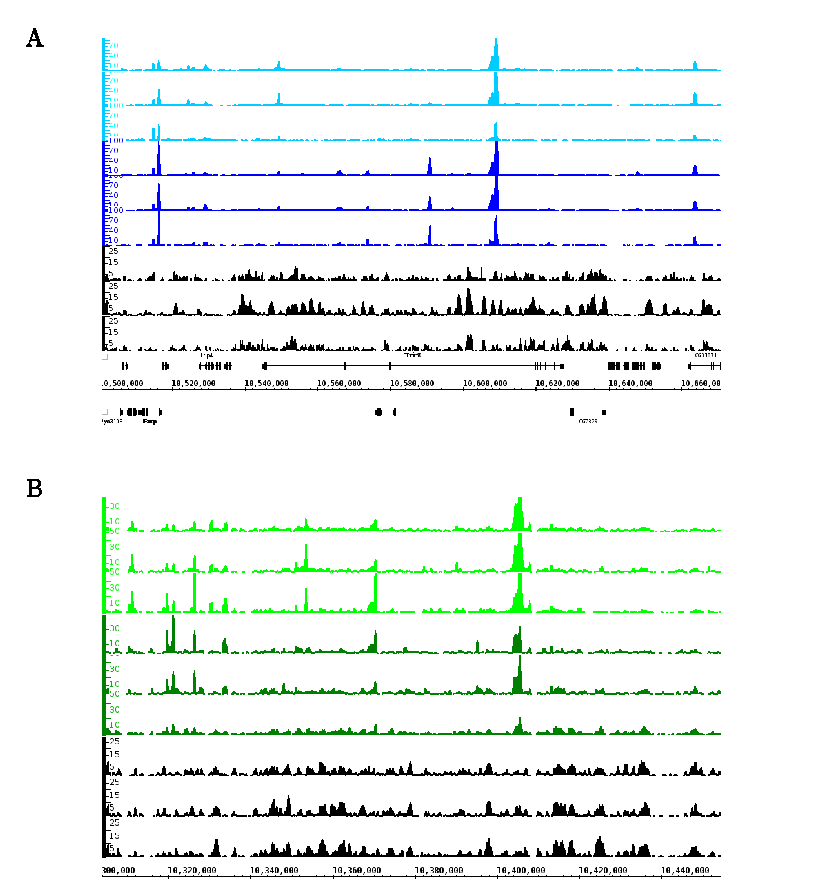
\includegraphics{fig4-1}
	\label{Figure 4.1}
\end{figure}

\begin{figure}[H]
\centering
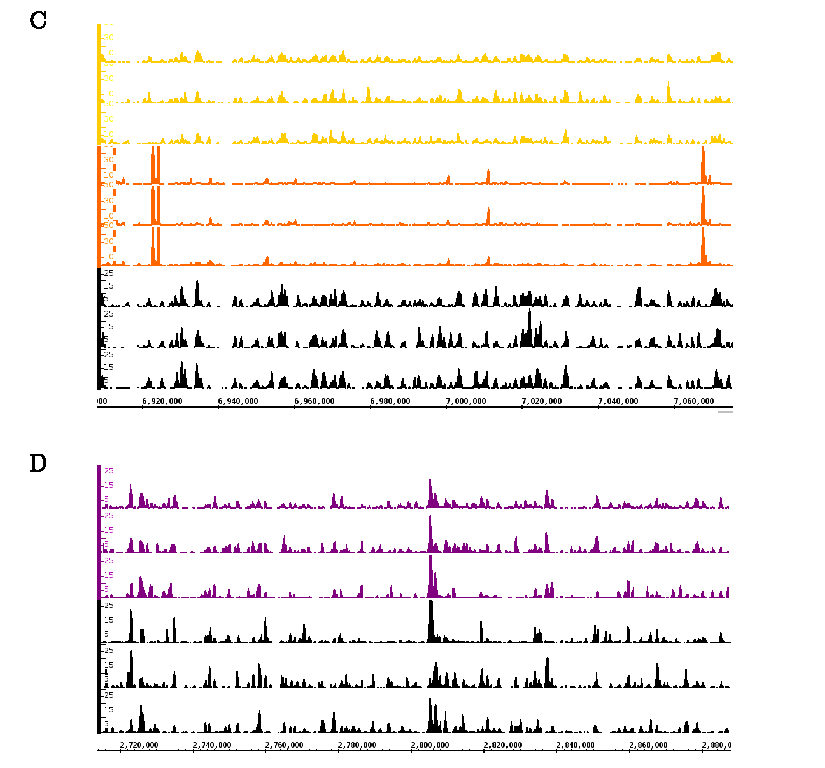
\includegraphics{fig4-1-1}
\caption{Reproducibility of biological replicate DamID samples. A.) \emph{D. melanogaster} samples. Shown is a 180-kb region of chromosome 2L; all other tracks in other species’ genomes show orthologous regions. The bottom three tracks (black) are the three Dam-only control replicates, the middle three tracks (blue) are the three Dichaete-Dam replicates, and the top three tracks (light blue) are the three SoxN-Dam replicates. B.) \emph{D. simulans} samples. The bottom three tracks (black) are the three Dam-only control replicates, the middle three tracks (green) are the three Dichaete-Dam replicates, and the top three tracks (light green) are the three SoxN-Dam replicates. C.) \emph{D. yakuba} samples. The bottom three tracks (black) are the three Dam-only control replicates, the middle three tracks (orange) are the three Dichaete-Dam replicates, and the top three tracks (light orange) are the three SoxN-Dam replicates. D.) \emph{D. pseudoobscura} samples. The bottom three tracks (black) are the three Dam-only control replicates, while the top three tracks (purple) are the three Dichaete-Dam replicates. All reads are scaled to a total library size of 1 million for visualization purposes. For \emph{D. melanogaster}, the y-axes of the Dichaete-Dam and SoxN-Dam tracks range from 0-100 reads, while for all other species they range from 0-50 reads. The y-axes of all Dam-only tracks range from 0-30 reads in order to show the structure of these samples more closely.}
\label{Figure 4.1}
\end{figure}

\begin{table}[!h]
\centering
\begin{tabular}{|l|l|l|l|}
\hline
\textbf{Sample}             & \textbf{Clean reads} & \textbf{Mapped reads} & \textbf{\% Duplicate reads} \\ \hline
\emph{D. mel} D-Dam 1*    & 3,524,222   & 2,957,450    & 34.3               \\ \hline 
\emph{D. mel} D-Dam 2     & 19,443,486  & 17,681,725   & 40.8               \\ \hline
\emph{D. mel} D-Dam 3     & 18,724,525  & 16,537,523   & 39.9               \\ \hline
\emph{D. mel} SoxN-Dam 1* & 3,878,298   & 3,381,641    & 20.6               \\ \hline
\emph{D. mel} SoxN-Dam 2  & 18,114,056  & 15,864,372   & 43.4               \\ \hline
\emph{D. mel} SoxN-Dam 3  & 17,125,196  & 15,799,860   & 48.9               \\ \hline
\emph{D. mel} Dam 1*      & 5,165,334   & 2,198,072    & 25.2               \\ \hline
\emph{D. mel} Dam 2*      & 8,699,134   & 3,379210     & 28.6               \\ \hline
\emph{D. mel} Dam 3       & 18,225,579  & 14,970,090   & 33.5               \\ \hline
\emph{D. sim} D-Dam 1     & 11,506,247  & 9,238,360    & 38.3               \\ \hline
\emph{D. sim} D-Dam 2     & 13,729,540  & 10,492,499   & 32.2               \\ \hline
\emph{D. sim} D-Dam 3     & 12,839,381  & 9,842,133    & 27.6               \\ \hline
\emph{D. sim} SoxN-Dam 1  & 10,571,945  & 8,607,660    & 40.9               \\ \hline
\emph{D. sim} SoxN-Dam 2  & 11,933,942  & 9,300,216    & 50.9               \\ \hline
\emph{D. sim} SoxN-Dam 3  & 10,962,128  & 9,531,855    & 34                 \\ \hline
\emph{D. sim} Dam 1       & 11,156,498  & 6,711,450    & 37.9               \\ \hline
\emph{D. sim} Dam 2       & 12,867,981  & 9,176644     & 32.5               \\ \hline
\emph{D. sim} Dam 3       & 12,351,232  & 9,719,920    & 30                 \\ \hline
\emph{D. yak} D-Dam 1     & 14,791,084  & 12,244,800   & 37.8               \\ \hline
\emph{D. yak} D-Dam 2     & 13,712,518  & 11,662,356   & 44.6               \\ \hline
\emph{D. yak} D-Dam 3     & 13,483,629  & 11,018,173   & 44.4               \\ \hline
\emph{D. yak} SoxN-Dam 1  & 14,262,567  & 7,448,087    & 37.4               \\ \hline
\emph{D. yak} SoxN-Dam 2  & 13,678,011  & 10,119,667   & 26.7               \\ \hline
\emph{D. yak} SoxN-Dam 3  & 13,781,619  & 5,824,891    & 36.6               \\ \hline
\emph{D. yak} Dam 1       & 12,258,054  & 7,544,899    & 29                 \\ \hline
\emph{D. yak} Dam 2       & 13,061,238  & 7,143,573    & 42.7               \\ \hline
\emph{D. yak} Dam 3       & 12,433,795  & 7,937,345    & 31.7               \\ \hline
\emph{D. pse} D-Dam 1     & 14,019,105  & 10,317,759   & 30.9               \\ \hline
\emph{D. pse} D-Dam 2     & 17,902,325  & 12,944,730   & 24.3               \\ \hline
\emph{D. pse} D-Dam 3     & 19,617,445  & 14,659,850   & 40                 \\ \hline
\emph{D. pse} Dam 1       & 19,261,105  & 12,015,266   & 45.2               \\ \hline
\emph{D. pse} Dam 2       & 12,857,397  & 8,001,867    & 37.2               \\ \hline
\emph{D. pse} Dam 3       & 19,170,000  & 11,769,256   & 43.3               \\ \hline
\end{tabular}
\caption{Summary of reads for DamID-seq experiments on the Illumina HiSeq 2000 and Illumina MiSeq. Abbreviations: \emph{D. mel, Drosophila melanogaster; D. sim, Drosophila simulans; D. yak, Drosophila yakuba; D. pse, Drosophila pseudoobscura}; D-Dam, Dichaete-Dam fusion protein; SoxN-Dam, SoxNeuro-Dam fusion protein; Dam, Dam-only control. * Samples sequenced on the MiSeq.}
\label{Table 4.1}
\end{table}

To facilitate the comparison of binding profiles for Dichaete-Dam and SoxN-Dam between \emph{D. melanogaster} and each other species, I used the UCSC LiftOver utility to translate the mapped reads from each of the three non-melanogaster species to the \emph{D. melanogaster} genome. It is possible to translate either the reads themselves or called binding intervals; I chose to do the translation at the read level to enable a more quantitative comparison of the binding profiles between species, as translating just the binding intervals results in loss of information about peak height and reproducibility between replicates \citep{bardet_computational_2011}. The translation process inevitably results in the loss of some reads, as not all genomic regions can be reliably translated to a single orthologous region in \emph{D. melanogaster}. The tradeoff between the number of reads successfully translated and the quality of the resulting translated regions can be controlled to some extent with the -minMatch parameter, which determines the percentage of base pairs in the original read that must re-map in order for the translated read to be reported. Following the recommendations of Bardet et al. \citet{bardet_computational_2011}, I used a minMatch value of 0.7 for translating \emph{D. simulans} and \emph{D. yakuba} reads to the \emph{D. melanogaster} genome. For \emph{D. pseudoobscura}, in order to account for the increasing phylogenetic distance and improve the percentage of translated reads, I used a minMatch value of 0.5.\\

The translated reads from each Sox fusion show broad similarities when plotted on the \emph{D. melanogaster} genome, although differences in binding profiles are visible, which increase with evolutionary distance. For Dichaete-Dam, the translated \emph{D. pseudoobscura} reads are considerably noisier and show fewer strong peaks than those of any other species (Figure 4.2A), while for SoxN-Dam, the translated \emph{D. yakuba} reads show fewer strong peaks than those of \emph{D. melanogaster} or \emph{D. simulans} (Figure 4.2B). Table 4.2 shows the number of translated reads for each dataset. Bardet \emph{et al.} (2011) calculated the percentages of all theoretical 36-bp reads that could be mapped in various species and then translated into the \emph{D. melanogaster} genome. The percentages of reads that were translated for my datasets in \emph{D. simulans} and \emph{D. yakuba} were slightly lower than the calculated values (95.85\% and 95.97\%, respectively); however, they were still high. The percentages of reads that were translated for my \emph{D. pseudoobscura} datasets were on average higher than the calculated value (61.33\%); this is likely because Bardet \emph{et al.} used a minMatch of 0.7 for \emph{D. pseudoobscura} read translation, while I used a less stringent value of 0.5.\\

\begin{table}[h]
\centering
\begin{tabular}{|l|l|l|l|}
\hline
\textbf{Sample}            & \textbf{Mapped reads} & \textbf{Translated reads} & \textbf{\% Translated} \\ \hline
\emph{D. sim} D-Dam 1    & 9,238,360    & 8,500,194        & 92            \\ \hline
\emph{D. sim} D-Dam 2    & 10,492,499   & 9,482,382        & 90.4          \\ \hline
\emph{D. sim} D-Dam 3    & 9,842,133    & 8,510,191        & 86.5          \\ \hline
\emph{D. sim} SoxN-Dam 1 & 8,607,660    & 7,922,971        & 92            \\ \hline
\emph{D. sim} SoxN-Dam 2 & 9,300,216    & 8,608,138        & 92.6          \\ \hline
\emph{D. sim} SoxN-Dam 3 & 9,531,855    & 8,575,810        & 90            \\ \hline
\emph{D. sim} Dam 1      & 6,711,450    & 5,833,352        & 87            \\ \hline
\emph{D. sim} Dam 2      & 9,176644     & 7,970,590        & 86.9          \\ \hline
\emph{D. sim} Dam 3      & 9,719,920    & 8,647,395        & 90            \\ \hline
\emph{D. yak} D-Dam 1    & 12,244,800   & 10,858,592       & 88.7          \\ \hline
\emph{D. yak} D-Dam 2    & 11,662,356   & 10,566,103       & 90.6          \\ \hline
\emph{D. yak} D-Dam 3    & 11,018,173   & 9,990,838        & 90.7          \\ \hline
\emph{D. yak} SoxN-Dam 1 & 7,448,087    & 6,655,088        & 89.4          \\ \hline
\emph{D. yak} SoxN-Dam 2 & 10,119,667   & 8,563,484        & 84.6          \\ \hline
\emph{D. yak} SoxN-Dam 3 & 5,824,891    & 5,039,416        & 86.5          \\ \hline
\emph{D. yak} Dam 1      & 7,544,899    & 6,699,792        & 88.8          \\ \hline
\emph{D. yak} Dam 2      & 7,143,573    & 6,404,045        & 89.6          \\ \hline
\emph{D. yak} Dam 3      & 7,937,345    & 7,067,736        & 89            \\ \hline
\emph{D. pse} D-Dam 1    & 10,317,759   & 7,751,401        & 75.1          \\ \hline
\emph{D. pse} D-Dam 2    & 12,944,730   & 9,770,702        & 75.5          \\ \hline
\emph{D. pse} D-Dam 3    & 14,659,850   & 8,428,062        & 57.5          \\ \hline
\emph{D. pse} Dam 1      & 12,015,266   & 9,068,101        & 75.5          \\ \hline
\emph{D. pse} Dam 2      & 8,001,867    & 6,119,021        & 76.5          \\ \hline
\emph{D. pse} Dam 3      & 11,769,256   & 8,974,292        & 76.3          \\ \hline
\end{tabular}
\caption{Reads translated from each sample in a non-\emph{melanogaster} species into the \emph{D. melanogaster} dm3 genome assembly. Abbreviations: \emph{D. mel, Drosophila melanogaster; D. sim, Drosophila simulans; D. yak, Drosophila yakuba; D. pse, Drosophila pseudoobscura}; D-Dam, Dichaete-Dam fusion protein; SoxN-Dam, SoxNeuro-Dam fusion protein.}
\label{Table 4.2}
\end{table}

\begin{figure}[H]
	\centering
	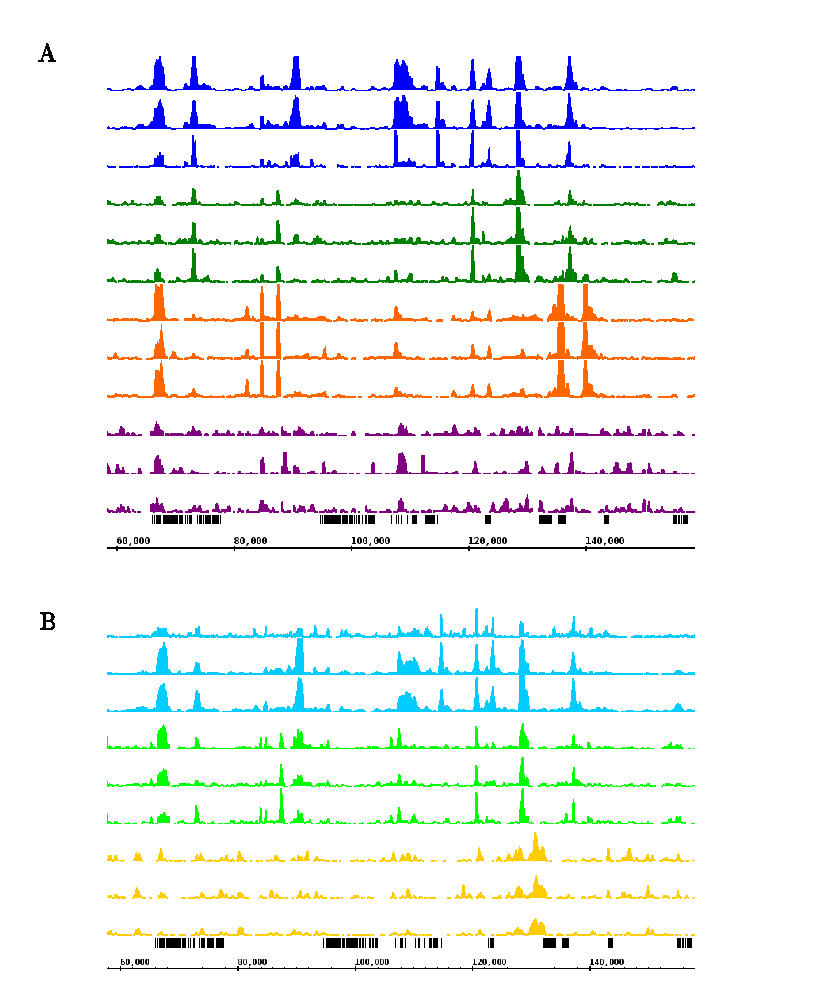
\includegraphics{fig4-2}
	\caption{Translated reads for Sox fusion proteins in all species. A.) Dichaete-Dam reads from all biological replicates in \emph{D. melanogaster} (blue), \emph{D. simulans} (green), \emph{D. yakuba} (orange) and \emph{D. pseudoobscura} (purple) are plotted on the \emph{D. melanogaster} genome. B.) SoxN-Dam reads from all biological replicates in \emph{D. melanogaster} (light blue), \emph{D. simulans} (light green) and \emph{D. yakuba} (light orange) are plotted on the \emph{D. melanogaster} genome. All reads are scaled to a total library size of 1 million after translation (if necessary) for visualization purposes. The y-axes of all tracks range from 0-50 reads. The same region of chromosome 2L is shown in both A and B.}
	\label{Figure 4.2}
\end{figure}

In order to detect regions of enriched binding by the Sox fusions in comparison to the Dam-only controls, I identified all GATC sites in each genome and then counted the number of reads mapping to each GATC fragment for each replicate. I then used DESeq2 to test for differential enrichment of Sox fusion reads versus the controls in each GATC fragment \citep{love_moderated_2014}. The log2 ratios between Sox fusion read counts and control read counts in each fragment represent normalized binding scores for each fusion protein, which were used in downstream analyses. Enriched fragments (adjusted p \textless 0.05) that were within 100 bp of each other were merged to create “peaks” or binding intervals; it should be noted that these binding intervals are different from ChIP peaks, as they are based on the distribution of GATC fragments across the genome. Because DESeq2 uses the variance observed between biological replicates to evaluate confidence for each potentially enriched interval, noisier data will result in fewer enriched binding intervals being called. This effect can be seen in the different numbers of binding intervals called for Dichaete-Dam in \emph{D. melanogaster, D. simulans} and \emph{D. yakuba} in comparison to \emph{D. pseudoobscura}, which had much noisier data. In \emph{D. yakuba}, although a high number of binding intervals were called for Dichaete-Dam, the SoxN-Dam experiment failed to detect significant binding. This result was surprising, since indications from the preliminary work seemed to show that both experiments worked equally well, and the same SoxN-Dam fusion protein showed high levels of binding in \emph{D. melanogaster} and \emph{D. simulans}. Visual inspection of the binding profiles for each fusion protein in \emph{D. yakub}a revealed that the SoxN-Dam replicates showed the same binding behavior as the Dam-only replicates (Figure 4.1C), suggesting that a mutation in the \emph{SoxN} sequence may have rendered the protein nonfunctional. All further analysis in \emph{D. yakuba} was performed with the Dichaete-Dam data only.\\

In \emph{D. melanogaster}, I also identified enriched intervals at a more stringent threshold, with an adjusted p-value \textless 0.01. For comparative analyses between species, I used the binding intervals identified at p \textless 0.05 in all species; however, for all subsequent functional analyses within \emph{D. melanogaster}, I used the more stringent p \textless 0.01 intervals. The numbers of binding intervals called for each fusion protein in each species can be seen in Table 4.3.\\

\begin{table}[h]
\centering
\begin{tabular}{|l|l|l|}
\hline
\textbf{Species}                           & \textbf{Dichaete-Dam} & \textbf{SoxNeuro-Dam} \\ \hline
\emph{D. melanogaster} p \textless 0.05  & 20848        & 22952        \\ \hline
\emph{D. melanogaster} p \textless 0.01  & 17530        & 17833        \\ \hline
\emph{D. simulans} p \textless 0.05      & 17833        & 17209        \\ \hline
\emph{D. yakuba} p \textless 0.05        & 26563        & 681          \\ \hline
\emph{D. yakuba} p \textless 0.01        & 21988        & 233          \\ \hline
\emph{D. pseudoobscura} p \textless 0.05 & 2951         & N/A          \\ \hline
\end{tabular}
\caption{Enriched binding intervals with indicated adjusted p-values called by DESeq2 for each fusion protein in each species. DamID for SoxNeuro-Dam was not performed in \emph{D. pseudoobscura}.}
\label{Table 4.3}
\end{table}

For each non-\emph{melanogaster} species, I also used the same procedure with the reads that had been translated to the \emph{D. melanogaster} genome assembly to detect differential binding by each Sox fusion in comparison to the Dam-only controls and to identify binding regions. This strategy resulted in binding intervals that were directly comparable to those identified in the \emph{D. melanogaster} DamID data; however, the total number of significantly enriched binding intervals called in the translated data decreased slightly in comparison to the number of binding intervals called in each species before translating reads (Table 4.4). I performed a crude pairwise comparison of the binding intervals detected in each species by intersecting the intervals called in \emph{D. melanogaster} with the intervals called in the translated data from each other species. Because more binding intervals were called in \emph{D. melanogaster} in most cases, the percentages of binding intervals present in \emph{D. melanogaster} that overlap with binding intervals in other species are generally lower than the percentages of binding intervals in each other species that overlap with binding intervals in \emph{D. melanogaster}. In \emph{D. yakuba}, a similar number of binding intervals were called for Dichaete-Dam as in \emph{D. melanogaster}. Accordingly, the percentages of overlapping intervals are very close for the two reciprocal comparisons. Considering the binding intervals in each non-\emph{melanogaster} species that overlap with intervals in \emph{D. melanogaster}, the percentages of shared intervals decrease with increasing phylogenetic distance, as expected \citep{he_high_2011,paris_extensive_2013}.\\

\begin{table}[h]
\begin{tabular}{|l|p{2cm}|p{2.5cm}|p{2.5cm}|p{2.5cm}|}
\hline
\textbf{Sample}          & \textbf{Binding intervals} & \textbf{Overlaps with \emph{D. mel} binding intervals} & \textbf{\% of \emph{D. mel} intervals overlapping} & \textbf{\% of non-\emph{D. mel} intervals overlapping} \\ \hline
\emph{D. sim} D-Dam    & 16119             & 11647                                  & 55.9                               & 72.3                                   \\ \hline
\emph{D. sim} SoxN-Dam & 15142             & 11891                                  & 51.8                               & 78.5                                   \\ \hline
\emph{D. yak} D-Dam    & 20964             & 14573                                  & 69.9                               & 69.5                                   \\ \hline
\emph{D. pse} D-Dam    & 2020              & 1301                                   & 6.24                               & 64.4                                   \\ \hline
\end{tabular}
\caption{Overlaps between binding intervals called on \emph{D. melanogaster} data and binding intervals called on translated read data. Abbreviations: \emph{D. mel, Drosophila melanogaster; D. sim, Drosophila simulans; D. yak, Drosophila yakuba; D. pse, Drosophila pseudoobscura}; D-Dam, Dichaete-Dam fusion protein; SoxN-Dam, SoxNeuro-Dam fusion protein.}
\label{Table 4.4}
\end{table}

\section{Functional analysis of binding patterns in each species}
\subsection{Overlap between DamID-seq binding intervals and core Sox binding intervals}
Previous work in the lab has generated a set of core binding intervals for both Dichaete and SoxN, based on a conservative integration of several ChIP-chip and DamID datasets for each transcription factor \citep{aleksic_role_2013,ferrero_soxneuro_2014}. In order to assess how well my binding data concur with these core intervals, I determined the overlaps between each of these datasets and the high-stringency DamID-seq binding intervals that I generated for each protein in \emph{D. melanogaster} (Table 4.5). Since the core interval datasets were the result of high-confidence overlaps between other datasets, they include fewer intervals than the DamID-seq datasets and should be more conservative. Accordingly, there is a higher proportion of core intervals that are overlapped by a DamID-seq interval than DamID-seq intervals that are overlapped by a core interval. While the levels of overlap between my binding intervals and the Dichaete core intervals were reasonably good, for SoxN they were considerably lower. However, the SoxN core intervals are, on average, shorter than the Dichaete core intervals, which could artificially lower the agreement between the datasets, as nearby but slightly offset binding intervals are less likely to actually overlap with small core intervals than large ones. Additionally, both the SoxN and Dichaete core intervals are derived from experiments using embryos that were collected over a narrower range of developmental stages than the DamID-seq experiments (stages 8-11 for SoxN DamID-chip, stages 7-10 and 11-13 for SoxN ChIP-chip, stages 5-11 for Dichaete DamID-chip, and stage 4-5 and 0-11 for Dichaete ChIP-chip), meaning that some binding sites detected by DamID-seq may not have been bound or accessible during the stages represented in the core intervals.\\ 

\begin{table}[h]
\centering
\begin{tabular}{|l|p{3cm}|p{4cm}|p{4cm}|}
\hline
              & \textbf{Core intervals} & \textbf{Core intervals containing DamID-seq intervals} & \textbf{DamID-seq intervals containing core intervals} \\ \hline
Dichaete core & 6720           & 4046 (60.2\%)                                 & 3774 (21.5\%)                                 \\ \hline
SoxN core     & 5482           & 1893 (34.5\%)                                 & 1683 (9.8\%)                                  \\ \hline
\end{tabular}
\caption{Overlaps between DamID-seq binding intervals and core binding intervals for Dichaete and SoxN in \emph{D. melanogaster} \citep{aleksic_role_2013,ferrero_soxneuro_2014}.}
\label{Table 4.5}
\end{table}

\subsection{Enriched motifs in binding intervals}
I performed a motif analysis on the binding intervals to identify enriched sequence motifs relative to the genomic background using HOMER \citep{heinz_simple_2010}. A \emph{de novo} motif analysis, which searches for any enriched 8-, 10- or 12-mers within binding intervals, uncovered a highly significantly enriched Dichaete motif (p = 1e-64) in the \emph{D. melanogaster} Dichaete-Dam intervals (Figure 4.3A) \citep{aleksic_role_2013}. Although the Dichaete motif was strongly enriched, it was the 14th ranked motif by p-value. The top 20 motifs identified by HOMER are listed in Table 4.6; these include a motif matching that of Ventral veins lacking (vvl, p = 1e-63), which is a known Dichaete cofactor in the midline \citep{aleksic_role_2013,soriano_drosophila_1998}.\\

\begin{table}[h]
\centering
\begin{tabular}{|l|l|l|l|}
\hline
\textbf{Rank} & \textbf{Transcription Factor} & \textbf{Consensus Sequence} & \textbf{P-value} \\ \hline
1    & Kni                  & GATCHAWT           & 1E-124  \\ \hline
2    & Ftz                  & CCAAGGAGACCG       & 1E-116  \\ \hline
3    & Run                  & TTGYGGCTACAW       & 1E-104  \\ \hline
4    & Tin                  & TCCACCCGAAAT       & 1E-096  \\ \hline
5    & Prd                  & TAGACGGTCT         & 1E-094  \\ \hline
6    & Sd                   & ACTCCATTTTGC       & 1E-094  \\ \hline
7    & Nub                  & TCCTTTGSATDT       & 1E-093  \\ \hline
8    & Usp                  & CGGGGTCAACTA       & 1E-092  \\ \hline
9    & Su(H)                & AGAATGTGAGTA       & 1E-091  \\ \hline
10   & CG11617              & TTTACATCCAGA       & 1E-086  \\ \hline
11   & Br                   & TCTATTTCTATA       & 1E-078  \\ \hline
12   & Kni                  & CGACCCSGTTTW       & 1E-078  \\ \hline
13   & Onecut               & ATTTAATCAATG       & 1E-072  \\ \hline
14   & D                    & CTACAATGGT         & 1E-064  \\ \hline
15   & Tag                  & TCTAACTYCA         & 1E-064  \\ \hline
16   & Vvl                  & ACTATCCACC         & 1E-063  \\ \hline
17   & Med                  & TCYCCGKCTGKC       & 1E-054  \\ \hline
18   & Abd-B                & GGTGGCCATSMA       & 1E-051  \\ \hline
19   & Tin                  & TGAACTCTTGAT       & 1E-050  \\ \hline
20   & Btd                  & TGGAGGCBGAAT       & 1E-048  \\ \hline
\end{tabular}
\caption{Top 20 \emph{de novo} motifs identified in p \textless 0.01 \emph{D. melanogaster} Dichaete-Dam intervals. The best match transcription factor, the consensus sequence, and the p-value are shown for each motif.}
\label{Table 4.6}
\end{table}

A \emph{de novo} motif analysis on the high-stringency SoxN-Dam intervals uncovered a significantly enriched match to a Dichaete motif (p = 1e-33), which was ranked 22nd by p-value. Additionally, the two top-scoring motifs were for Pangolin (Pan), a transcription factor that also contains an HMG box DNA binding domain. When I performed the same analysis on the high-stringency intervals before merging, so that the same sequences were considered but they were broken up into a greater number of fragments, a stronger match to a Dichaete motif was discovered, ranking 9th by p-value (Figure 4.3B, p = 1e-84); this motif was present in 16.8\% of target sequences, a far greater percentage than for most other enriched motifs. It is also highly similar to the SoxN motif reported in an independent DamID experiment in \emph{D. melanogaster} \citep{ferrero_soxneuro_2014}. The top 20 motifs identified by HOMER in the unmerged intervals are listed in Table 4.7. For both Dichaete-Dam and SoxN-Dam, the top motif was predicted by HOMER to match Kni; however, since this motif contains the sequence GATC in both cases, it is likely the presence of this motif is due to the fact that the interval boundaries were determined by GATC sites, rather than reflecting true Kni binding.\\

\begin{table}[h]
\centering
\begin{tabular}{|l|l|l|l|}
\hline
\textbf{Rank} & \textbf{Transcription Factor} & \textbf{Consensus Sequence} & \textbf{P-value} \\ \hline
1    & Kni                  & ATCCGATC           & 1e-859  \\ \hline
2    & Tll                  & TTGCAACGTTAA       & 1E-162  \\ \hline
3    & Twi                  & CGCATATGCGAT       & 1E-143  \\ \hline
4    & Trl                  & AGAGTAGTKCCA       & 1E-135  \\ \hline
5    & Eip74EF              & GGGAGAATTHTG       & 1E-127  \\ \hline
6    & Brk                  & MGTGCCSC           & 1E-112  \\ \hline
7    & B-H2                 & TGCCTATTAAST       & 1E-101  \\ \hline
8    & Slp1                 & GTCAATATTTAC       & 1E-090  \\ \hline
9    & D                    & CCTTTGTT           & 1E-084  \\ \hline
10   & Ap                   & GCCGCTAATCAG       & 1E-082  \\ \hline
11   & Hb                   & TTTTTTTTTTTT       & 1E-082  \\ \hline
12   & Med                  & CATAYTGCGS         & 1E-074  \\ \hline
13   & TATA-box             & TTATAGGGAG         & 1E-073  \\ \hline
14   & Antp                 & YATAWTATRGGN       & 1E-072  \\ \hline
15   & Bap                  & TCTTGTTTAAGT       & 1E-071  \\ \hline
16   & Slbo                 & CTCWGTTGCTTG       & 1E-070  \\ \hline
17   & Antp                 & ATTCTGATTTGT       & 1E-060  \\ \hline
18   & Kni                  & AWATGGATCCAT       & 1E-057  \\ \hline
19   & Cad                  & CATAAAGA           & 1E-053  \\ \hline
20   & Trl                  & CACGACAGAG         & 1E-053  \\ \hline
\end{tabular}
\caption{Top 20 \emph{de novo} motifs identified in unmerged p \textless 0.01 \emph{D. melanogaster} SoxN-Dam intervals. The best match transcription factor, the consensus sequence, and the p-value are shown for each motif.}
\label{Table 4.7}
\end{table}

For all other species, I used HOMER to search for motifs in the binding intervals called in the original genomes, rather than in the intervals called after translation to the \emph{D. melanogaster} genome. I used the sequences from each original genome because they contained the sites to which the fusion proteins actually bound \emph{in vivo}, and also because any differences in the enriched motifs found between species might illustrate general differences in enhancer composition. In the \emph{D. simulans} binding intervals, a \emph{de novo} motif analysis of the Dichaete-Dam data uncovered a significantly enriched motif (p = 1e-20) matching the Sox consensus binding sequence (Figure 4.3C) ranked in the 23rd position by p-value. Other highly-ranked motifs included matches to Tll (p = 1e-30) and Kni (p = 1e-29). Additionally, a search for known motifs resulted in three hits to Sox motifs, corresponding to the vertebrate Sox2 (p = 1e-12), Sox3 (p = 1e-15) and Sox6 (p = 1e-13) motifs. A de novo motif analysis of the \emph{D. simulans} SoxN-Dam binding intervals discovered a Sox motif as the 2nd-ranked enriched motif (Figure 4.3D, p = 1e-37), and a search for known motifs also resulted in hits for the vertebrate Sox2 (p = 1e-24), Sox3 (p = 1e-32) and Sox6 (p = 1e-25) motifs. Other high-ranking motifs included Pan (p = 1e-37) and Zeste (z, p = 1e-23), with matches to Vvl (p = 1e-17) and Tll (p = 1e-15) being found further down the list, at positions 24 and 27.\\

In \emph{D. yakuba}, a \emph{de novo} motif search of the Dichaete-Dam binding intervals uncovered a significantly enriched motif (p = 1e-39) matching the vertebrate Sox2 motif (Figure 4.3E), which was the 4th ranked motif by p-value and was present in 12.01\% of target sequences. Other high-ranked motifs included Glial cells missing (Gcm, p = 1e-39), Tll (p = 1e-35), Slow border cells (Slbo, p = 1e-36), Ventral nervous system defective (Vnd, p = 1e-35) and Vvl (p = 1e-35). Additionally, a search for known motifs identified a Sox6 motif (p = 1e-21) and a Sox3 motif (p = 1e-17) as the top two hits, with a Sox2 motif as the 6th-ranked hit (p = 1e-9).\\

Although a relatively small number of binding intervals were called for Dichaete-Dam in \emph{D. pseudoobscura}, they still show enrichment for Sox motifs. A \emph{de novo} motif search identified a significantly enriched motif (p = 1e-8) whose best match is to the vertebrate Sox9 motif (Figure 4.3F). Performing the same \emph{de novo} search on the binding intervals before merging also uncovered a Sox9 motif; however, in this case the motif was a stronger match and had a lower p-value (p = 1e-21), as well as being present in a greater proportion of target sequences (29.53\% versus 1.16\% for the merged intervals). Other high-ranked motifs included Deformed epidermal autoregulatory factor-1 (Deaf1, p = 1e-32), Twi (p = 1e-23), Vnd (p = 1e-21) and Trl (p = 1e-18). For both the merged and unmerged intervals, a search for known motifs turned up the vertebrate Sox2 (p = 1e-7), Sox3 (p = 1e-6) and Sox6 (p = 1e-5) motifs as the top three hits.\\

\begin{figure}[ht]
	\centering
	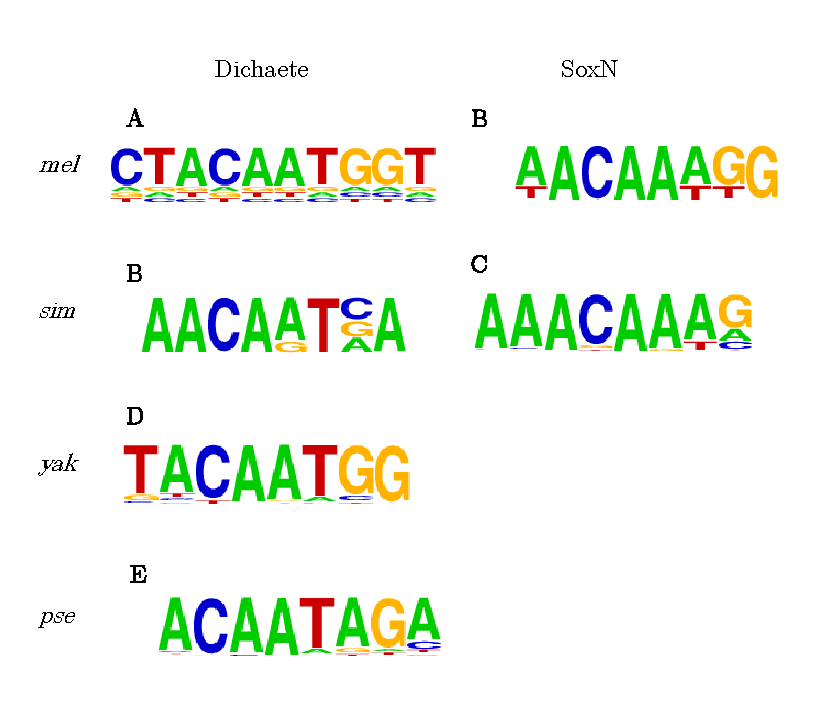
\includegraphics{fig4-3}
	\caption{\emph{De novo} Sox motifs discovered in DamID binding intervals. A.) Sox motif discovered in \emph{D. melanogaster} Dichaete-Dam intervals. B.) Sox motif discovered in \emph{D. melanogaster} SoxN-Dam intervals. C.) Sox motif discovered in \emph{D. simulans} Dichaete-Dam intervals. D.) Sox motif discovered in \emph{D. simulans} SoxN-Dam intervals. E.) Sox motif discovered in \emph{D. yakuba} Dichaete-Dam intervals. F.) Sox motif discovered in \emph{D. pseudoobscura} Dichaete-Dam intervals.}
	\label{Figure 4.3}
\end{figure}

The binding site analysis supports the view that the DamID experiments have identified genomic regions bound by Dichaete and SoxNeuro in vivo. Unlike ChIP-seq peaks, DamID-seq binding intervals are dependent on the distribution of GATC sites across the genome; as a result, they may contain flanking sequences that are not relevant to the factor-specific binding sites and thus lower target motif enrichments are expected. Although some sets of binding intervals, such as those for SoxN-Dam in \emph{D. simulans}, show higher enrichment for Sox motifs than others, the fact that at least one Sox motif was identified in each dataset is encouraging. It is known that Dichaete and SoxN recognize very similar sequence motifs to the canonical Sox motif, A/T A/T CAAAG, a fact which is supported by my data \citep{aleksic_role_2013,ferrero_soxneuro_2014}. However, when comparing across species, certain patterns of preferences become visible; most clearly, in all four species assayed, the Sox motif found in Dichaete binding intervals contains a stronger match to a thymine residue at the fourth position of the core “CAAAG” motif, while each Sox motif found in SoxN binding intervals contains a stronger match to an adenine residue in that position (Figure 4.3). Additional motifs for transcription factors that have been shown to interact with both Dichaete and SoxN, such as Vvl, Vnd, Tll and Nub \citep{aleksic_role_2013,ferrero_soxneuro_2014,soriano_drosophila_1998}, were also discovered in binding intervals, as well as motifs for other developmentally-important TFs. Finally, the motif for Trl, which was enriched in several binding datasets and has previously been shown to be associated with Dichaete binding \citep{aleksic_role_2013}, is also a signature of highly occupied target (HOT) regions in the \emph{Drosophila} genome, which are regions at which many TFs are reported to bind \citep{kvon_hot_2012}. Taken together, these results suggest that the Dichaete-Dam and SoxN-Dam binding intervals identify active and developmentally-relevant enhancers.

\subsection{Gene and genomic annotation of binding intervals}
I assigned each binding interval to the closest gene in the \emph{D. melanogaster} genome within 10 kb upstream or downstream, using the intervals called on translated reads for all non-\emph{melanogaster} species and the gene annotations from FlyBase release 5.55. A summary of the numbers of genes annotated to each dataset, as well as the number of genes that were commonly annotated to Dichaete-Dam binding intervals and SoxN-Dam binding intervals in \emph{D. melanogaster} and \emph{D. simulans}, can be seen in Table 4.8. In both species, a high percentage of all target genes are shared between the two TFs, although this percentage is slightly higher in \emph{D. melanogaster} than in \emph{D. simulans} (89\% of Dichaete-Dam targets and 88\% of SoxN-Dam targets versus 80\% of Dichaete-Dam targets and 84\% of SoxN-Dam targets).\\

Combining previous ChIP-chip and DamID experiments with gene expression experiments has allowed us to identify direct targets of both Dichaete and SoxN in \emph{D. melanogaster}; for Dichaete, this includes 1373 genes, while for SoxN it includes 544. I determined the number of these direct targets that are included in the genes annotated to each DamID-seq binding dataset. I also found the overlaps between genes annotated to the core binding intervals for each TF and the genes annotated to each DamID-seq dataset. A high percentage (70-90\%) of both direct target genes and core interval genes are included in the gene annotations for Dichaete-Dam and SoxN-Dam binding intervals in all species but \emph{D. pseudoobscura}. In both \emph{D. melanogaster} and \emph{D. simulans}, a slightly higher percentage of direct target and core interval genes are also annotated to the Dichaete-Dam binding intervals than to SoxN-Dam binding intervals. Among all the Dichaete-Dam datasets, the genes annotated to intervals translated from \emph{D. yakuba} contain the most core interval genes and direct target genes; this is likely because the \emph{D. yakuba} Dichaete-Dam intervals had the largest number of gene annotations overall. These results shows good concordance between both the core and direct target genes for each TF and the DamID-seq target genes in all species, with the exception of \emph{D. pseudoobscura}, which had a much lower number of binding intervals and target genes.\\

\begin{table}[h]
\centering
\begin{tabular}{|l|p{2cm}|p{2cm}|p{2.5cm}|p{2.5cm}|}
\hline
\textbf{Dataset}         & \textbf{Genes annotated to binding intervals} & \textbf{Genes common to Dichaete and SoxN} & \textbf{Core interval genes annotated to binding intervals} & \textbf{Direct target genes annotated to binding intervals} \\ \hline
\emph{D. mel} D-Dam    & 9400                                 & 8445                              & 3433/4279 (80.2\%)                                 & 1173/1373 (85.4\%)                                 \\ \hline
\emph{D. mel} SoxN-Dam & 9528                                 & 8445                              & 2410/3246 (74.2\%)                                 & 434/544 (80.0\%)                                   \\ \hline
\emph{D. sim} D-Dam    & 9383                                 & 7524                              & 3228/4279 (75.4\%)                                 & 1111/1373 (80.9\%)                                 \\ \hline
\emph{D. sim} SoxN-Dam & 8948                                 & 7524                              & 2326/3246 (71.7\%)                                 & 412/544 (80.0\%)                                   \\ \hline
\emph{D. yak} D-Dam    & 12192                                & N/A                               & 3765/4279 (88.0\%)                                 & 1249/1373 (91.0\%)                                 \\ \hline
\emph{D. pse} D-Dam    & 1888                                 & N/A                               & 978/4279 (22.9\%)                                  & 407/1373 (29.6\%)                                  \\ \hline
\end{tabular}
\caption{Gene annotations for DamID-seq binding intervals. Numbers of genes common to Dichaete-Dam and SoxN-Dam are within each species. For core interval genes and direct target genes, shown are numbers annotated to intervals in each DamID-seq dataset over total number of core or direct target genes. Abbreviations: \emph{D. mel, Drosophila melanogaster; D. sim, Drosophila simulans; D. yak, Drosophila yakuba; D. pse, Drosophila pseudoobscura}; D-Dam, Dichaete-Dam fusion protein; SoxN-Dam, SoxNeuro-Dam fusion protein.}
\label{Table 4.8}
\end{table}

I performed enrichment analyses for Gene Ontology Biological Process (GO:BP) terms annotated to the genes hit by each TF in each species. In line with previous studies of Dichaete and SoxN binding \citep{aleksic_role_2013,ferrero_soxneuro_2014}, targets of both TFs were highly enriched for general terms relating to organ and system development (p \textless 1e-47) and biological regulation (p \textless 1e-44). They were also both enriched for imaginal disc development (p \textless 1e-19), generation of neurons (p \textless 1e-29) and regulation of transcription (p \textless 1e-9). Enriched terms for both proteins were highly similar across species (Appendix X). Notably, although there were many less genes hit by Dichaete-Dam in \emph{D. pseudoobscura} than in the other species, the genes that were hit showed strong enrichment for similar GO:BP terms as in the other species, were strongly upregulated in the brain and larval CNS, and were highly associated with publications describing genes involved in the neural stem cell transcriptional network (p \textless 1e-25), all of which are hallmarks of known Dichaete function \citep{aleksic_role_2013,shen_identifying_2013,soriano_drosophila_1998}.\\ 

Using the same gene assignments, I calculated the distances between the end of each binding interval that was closest to each assigned gene and the transcription start site (TSS) of each gene to which it was assigned. It should be noted that, because DamID is dependent on the non-random distribution of GATC sites across the genome, it is difficult to know where a true binding site is located within a binding interval. Consequently, the distances between binding intervals and genomic features may not always accurately reflect the distances between the actual binding sites and those intervals. Nonetheless, they give an overview of where the DamID-fusion proteins bind relative to genes. I plotted these distances using the ChIPseeker R package (Figure 4.4) (cite ChIPseeker R package).\\ 

\begin{figure}
\centering
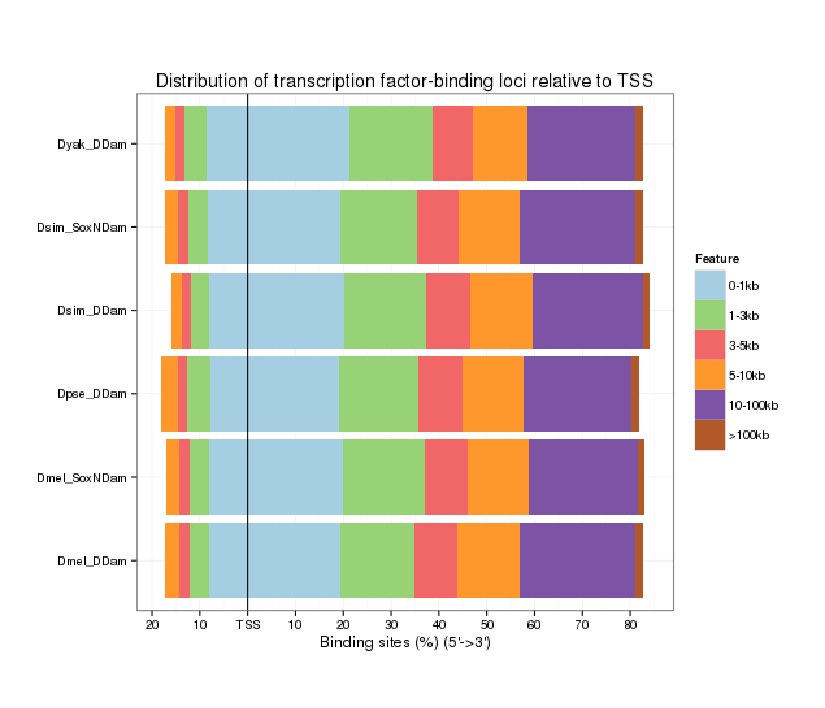
\includegraphics{fig4-4}
\caption{Distribution of Sox DamID binding intervals around TSS of annotated genes for each dataset. Distances were calculated from the end of each interval closest to its annotated gene (upstream or downstream). Sox DamID binding shows a clear skew towards positions downstream of TSSs.}
\label{Figure 4.4}
\end{figure}

The overall distribution of distances is very similar for each transcription factor in each species. Although around 30\% of binding intervals are located within 1 kb up- or downstream of TSSs, there is a clear skew towards downstream locations, suggesting a high amount of binding to regulatory regions in introns. Approximately 75\% of binding intervals are located within 10 kb of the TSS in either direction, with the remaining ~25\% being located more distally downstream. I also used a custom pipeline in R (CHIPPAVI, Bettina Fischer) to plot the probability density of bound nucleotides around all TSSs; these plots used gene annotations following the same behavior as previously but with no upper limit on the distance between an interval and the closest nearby gene (Figure 4.5). These plots show a strong maximum at the TSS, with a skew towards downstream binding, although the skew is less pronounced than with the ChIPseeker plots. The distribution of binding around TSSs is very similar for both Dichaete and SoxN and across all species, although the plots for Dichaete-Dam in \emph{D. pseudoobscura} are less smooth due to the lower number of binding intervals.\\

\begin{figure}
	\centering
	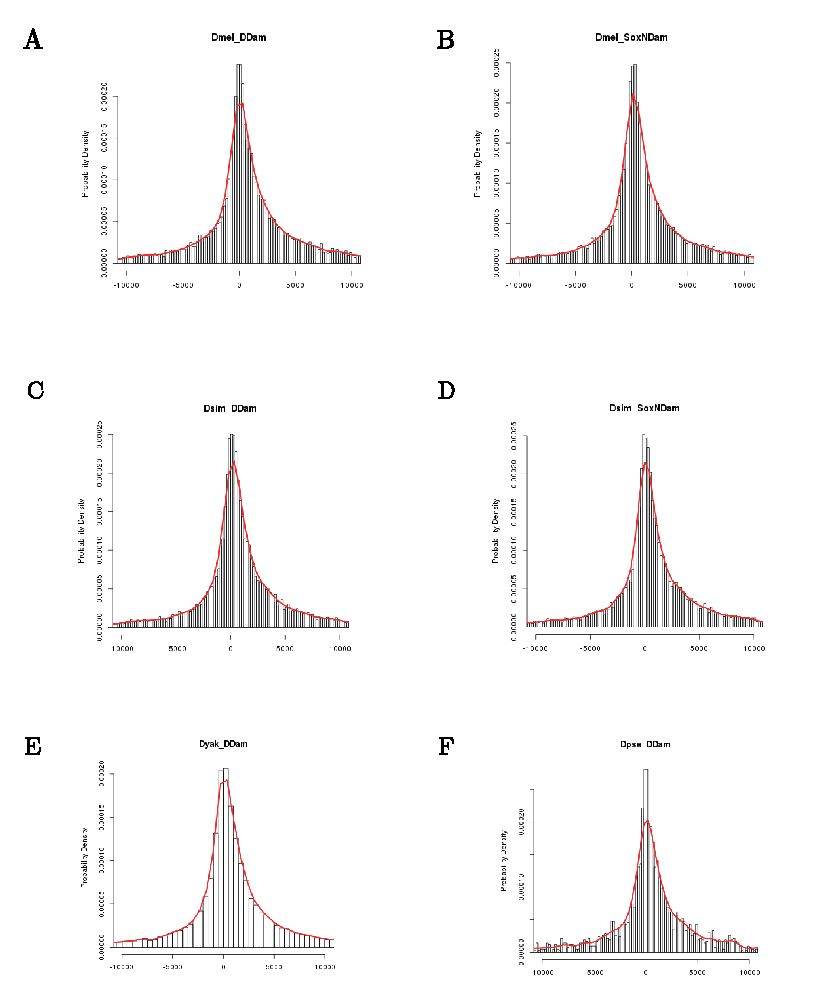
\includegraphics{fig4-5}
	\caption{Distribution of Sox DamID binding intervals around TSSs for all genes in the \emph{D. melanogaster} genome. A.) Probability density of bound nucleotides around TSSs for \emph{D. melanogaster} Dichaete-Dam. B.) Probability density of bound nucleotides around TSSs for \emph{D. melanogaster} SoxN-Dam. C.) Probability density of bound nucleotides around TSSs for \emph{D. simulans} Dichaete-Dam. D.) Probability density of bound nucleotides around TSSs for \emph{D. simulans} SoxN-Dam. E.) Probability density of bound nucleotides around TSSs for \emph{D. yakuba} Dichaete-Dam. F.) Probability density of bound nucleotides around TSSs for \emph{D. pseudoobscura} Dichaete-Dam.}
	\label{Figure 4.5}
\end{figure}

I also annotated each binding interval in each dataset to a genomic feature category (exon, intron, 5’ UTR, 3’ UTR, promoter, immediate downstream, or intergenic) using the ChIPpeakAnno R package \citep{zhu_chippeakanno:_2010}. Each interval could be annotated to multiple categories if it overlapped an annotated region corresponding to more than one feature (e.g. an interval partially overlapping an intron and an exon would be annotated to both). Again, the overall pattern of genomic feature annotation is quite similar for each transcription factor in each species. The most often hit feature is introns, which are hit by approximately 65\% of binding intervals, followed by exons, which are hit by approximately 55\% of binding intervals (Figure 4.6A-F). This is in agreement with the TSS distance distributions, which indicate that the majority of binding intervals are located downstream of TSSs. Approximately 30\% of binding intervals are annotated to promoters. A higher percentage of the \emph{D. yakuba} intervals (64\%) are annotated to exons than in the other species. In \emph{D. pseudoobscura}, a higher percentage of intervals are annotated to intergenic regions than in other species, while lower percentages of intervals are annotated to exons, introns, and UTRs. However, considering the differing quality of the \emph{D. pseudoobscura} data and the lower number of intervals compared to the other species, it is difficult to interpret this as a biologically significant difference. In general, the patterns of binding to genomic features by Dichaete and SoxN appear very similar in all species studied.

\begin{figure}
	\centering
	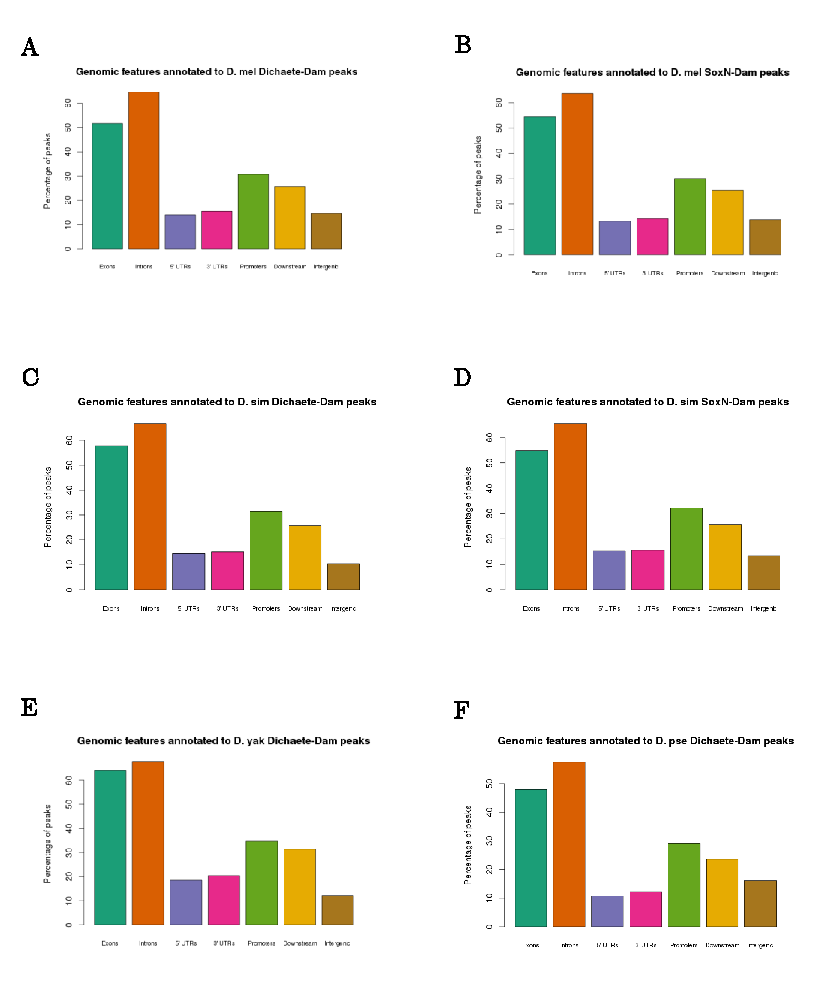
\includegraphics{fig4-6}
	\caption{Genomic features annotated to Sox DamID binding intervals. Feature classes include exons, introns, 5’ UTRs, 3’ UTRs, promoters, immediate downstream and intergenic. A.) Percentages of \emph{D. melanogaster} Dichaete-Dam intervals annotated to each genomic feature class. B.) Percentages of \emph{D. melanogaster} SoxN-Dam intervals annotated to each genomic feature class. C.) Percentages of \emph{D. simulans} Dichaete-Dam intervals annotated to each genomic feature class. D.) Percentages of \emph{D. simulans} SoxN-Dam intervals annotated to each genomic feature class. E.) Percentages of \emph{D. yakuba} Dichaete-Dam intervals annotated to each genomic feature class. F.) Percentages of \emph{D. pseudoobscura} Dichaete-Dam intervals annotated to each genomic feature class.}
	\label{Figure 4.6}
\end{figure}

\subsection{High overlap with known enhancers}
There are several resources containing data on known \emph{Drosophila} enhancers or \emph{cis}-regulatory elements (CRMs), based on a variety of different types of experimental evidence. I downloaded enhancers from REDFly, which contains 1864 manually-curated CRMs, and from the Janelia FlyLight database, which contains 7113 enhancers experimentally shown to drive expression of a GAL4 reporter construct in \emph{D. melanogaster} embryos, including 4724 with specific activity in the embryonic CNS \citep{,gallo_redfly_2010,manning_resource_2012}. I used the BEDTools suite to find the overlaps between the high-confidence Dichaete-Dam and SoxN-Dam intervals in \emph{D. melanogaster} and the annotated enhancers from each of these resources. I found that Dichaete-Dam and SoxN-Dam binding intervals overlap with a high number of REDFly and FlyLight enhancers (Table 4.9), with a slightly greater proportion of CNS-specific FlyLight enhancers containing Dichaete or SoxN binding than for all embryonic enhancers. Overall, more enhancers from each resource contain Dichaete binding than SoxN binding, although a large fraction of all bound enhancers are bound by both Dichaete and SoxN. Although the DamID binding intervals do not correspond directly to enhancer elements, since their borders are dependent on the genomic locations of GATC sites, in certain cases visual inspection reveals a remarkably high correlation between annotated enhancers and peaks of DamID binding, such as at the \emph{ind}, \emph{vnd}, \emph{dpp}, \emph{lola} and \emph{psq} loci (Figure 4.7). The highest overlaps are with the REDFly enhancers, which is encouraging considering that these enhancers have been curated using multiple supporting forms of evidence and can therefore be considered to be the highest-confidence dataset.\\

\begin{figure}
\centering
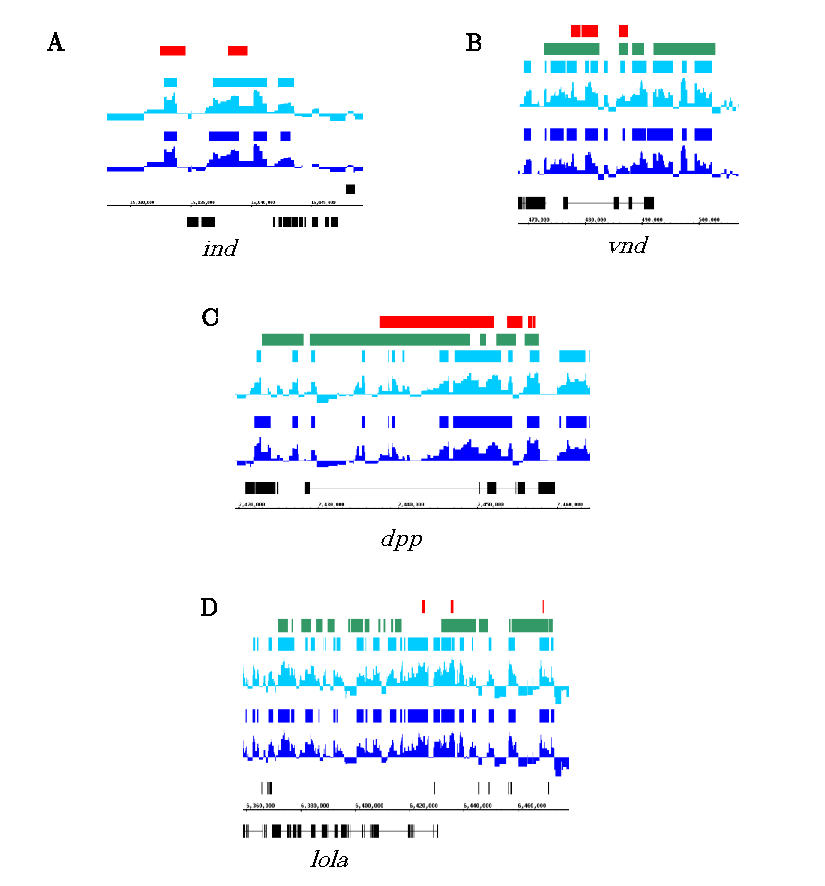
\includegraphics{fig4-7}
\caption{Concordance between \emph{D. melanogaster} Sox DamID binding intervals and known enhancers from REDFly and FlyLight. Binding profiles represent the normalized log2 fold changes between Sox fusion binding and Dam-only control binding in each GATC fragment. Dichaete-Dam binding profiles and intervals are in blue, SoxN-Dam binding profiles and intervals are in light blue, REDFly enhancers are in red and FlyLight enhancers are in green. A.) Overlaps between Dichaete-Dam and SoxN-Dam binding intervals and two REDFly enhancers at the \emph{ind} locus. B.) Overlaps between Dichaete-Dam and SoxN-Dam binding intervals and several REDFly and FlyLight enhancers at the \emph{vnd} locus. C.) Overlaps between Dichaete-Dam and SoxN-Dam binding intervals and several REDFly and FlyLight enhancers at the \emph{dpp} locus. D.) Overlaps between Dichaete-Dam and SoxN-Dam binding intervals and several REDFly and FlyLight enhancers at the \emph{lola} and \emph{psq} loci.}
\label{Figure 4.7}
\end{figure}

\begin{table}[h]
\centering
\begin{tabular}{|l|l|p{2.5cm}|p{2.5cm}|p{2.5cm}|}
\hline
              & \textbf{Enhancers} & \textbf{Enhancers overlapping with Dichaete binding} & \textbf{Enhancers overlapping with SoxN binding} & \textbf{Enhancers overlapping with Dichaete and SoxN binding} \\ \hline
REDFly        & 1864      & 1152 (61.8\%)                               & 1130 (60.6\%)                           & 1108 (59.4\%)                                        \\ \hline
FlyLight      & 7113      & 2999 (42.2\%)                               & 2784 (39.1\%)                           & 2681 (37.8\%)                                        \\ \hline
FlyLight CNS  & 4724      & 2077 (44.0\%)                               & 1935 (41.0\%)                           & 1857 (39.3\%)                                        \\ \hline
STARR-seq S2  & 2325      & 1092 (47.0\%)                               & 951 (40.9\%)                            & 912 (39.2\%)                                         \\ \hline
STARR-seq OSC & 3341      & 1144 (34.2\%)                               & 1061 (31.8\%)                           & 973 (29.1\%)                                         \\ \hline
\end{tabular}
\caption{Overlaps between Dichaete and SoxN binding and known enhancers in \emph{D. melanogaster}. Numbers in parentheses are percentages of all enhancers of each category containing specified binding.}
\label{Table 4.9}
\end{table}

In addition to the enhancers in these databases, I downloaded peak calls from a STARR-seq assay that was recently performed to identify enhancer activity in both S2 cells and ovarian somatic cells (OSCs) using DNA libraries from \emph{D. melanogaster, D. yakuba, D. ananassae, D. pseudoobscura} and \emph{D. willistoni} \citep{arnold_quantitative_2014}. These data include both low-stringency, unfiltered peaks, where any enhancer activity was detected, as well as high-stringency, thresholded peaks, where at least a 3-fold enrichment was observed in the STARR-seq samples compared to the input samples. The STARR-seq data contains peaks called for two independent replicates in each condition as well as peaks called for merged replicate data. To get a summary of high-confidence STARR enhancer activity, I focused on the thresholded, merged peaks from both S2 cells and OSCs. This is in line with the analysis of Arnold \emph{et al.}, who first showed that the independent replicates had high levels of reproducibility and then performed further analysis on merged data \citet{arnold_quantitative_2014}. The peaks were reported as summits; that is, the single genomic coordinate corresponding to the highest point of enrichment for each peak. Following the analysis from Arnold \emph{et al.}, I converted them to intervals by extending the coordinates 250 bp in either direction from the summits, resulting in 501-bp peaks. These enhancer peaks show a comparable overlap with Dichaete and SoxN binding as the FlyLight enhancers, with, again, a slightly greater percentage overlapping with Dichaete binding intervals than with SoxN binding intervals (Table 4.9).\\

It is interesting to note that, while a higher fraction of the S2 enhancer set is overlapped by Dichaete or SoxN binding intervals than with the OSC enhancers, in terms of absolute numbers this trend is reversed. The enhancers containing DamID-seq binding in the two cell types are mostly different; only 314 Dichaete-bound enhancers and 282 SoxN-bound enhancers are shared between S2 cells and OSCs. Although S2 cells are derived from an embryonic, haemocyte-like lineage, like OSCs they represent a specific, differentiated cell type. The DamID-seq binding intervals are derived from whole embryos containing diverse cell types over a wide range of developmental stages, meaning that they likely represent a regulatory landscape with both similarities to and differences from that of either S2 cells or OSCs. Therefore, it is not surprising that some DamID binding intervals would fall within enhancers characterized in the two different cell types, or that some would not overlap with any active enhancers in either S2 cells or OSCs.\\

Most of the enhancers characterized in the FlyLight and REDFly databases are considerably longer than 500 bp; it is therefore likely that the overlaps between the 501-bp STARR enhancers and the DamID-seq binding intervals are overly conservative. It is possible that some binding intervals that fall just outside of a 501-bp STARR enhancer are still located within a broader cis-regulatory region corresponding to that enhancer. In order to address this issue, I assigned all Dichaete-Dam and SoxN-Dam binding intervals to the nearest unfiltered STARR-seq peak (56220 in S2 cells and 44601 in OSCs). I then filtered the list of intervals to contain only those that are up to 1 kb away from the nearest peak. I also filtered out any STARR-seq peaks with a p-value greater than 0.001, resulting in a list of binding intervals assigned to nearby peaks that are high-confidence but include strong as well as weak enhancer activity. For Dichaete, this resulted in 2799 assignments in S2 cells, representing 16.0\% of high-confidence binding intervals, and 2662 assignments in OSCs, representing 15.2\% of high-confidence binding intervals. 1314 binding intervals were assigned to enhancers in both S2 cells and OSCs, while 1485 were only assigned to enhancers in S2 cells and 1348 were only assigned to enhancers in OSCs, bringing the total number of unique binding intervals assigned to an enhancer to 4147, or 23.7\% of high-confidence binding intervals. For SoxN, it resulted in 2663 assignments in S2 cells, representing 15.0\% of high-confidence binding intervals, and 2693 assignments in OSCs, representing 15.1\% of high-confidence binding intervals. 1167 binding intervals were assigned to enhancers in both S2 cells and OSCs, while 1496 were only assigned to enhancers in S2 cells and 1526 were only assigned to enhancers in OSCs, resulting in a total of 4189 unique intervals assigned to an enhancer, or 23.5\% of high-confidence binding intervals (Table 4.11).\\

STARR-seq was also performed with the \emph{D. yakuba} and \emph{D. pseudoobscura} genomes in S2 cells and, in the case of \emph{D. yakuba}, in OSCs. As with \emph{D. melanogaster}, I found the overlaps between the Dichaete-Dam binding intervals and 501-bp peaks around each STARR-seq summit in each species (Table 4.10). In contrast to the \emph{D. melanogaster} data, the \emph{D. yakuba} Dichaete-Dam intervals overlap with a much higher percentage of STARR-seq enhancers in S2 cells than in OSCs, although in absolute numbers they still overlap more OSC enhancers. The overlap percentages are also higher overall in \emph{D. yakuba}; however, it is difficult to draw conclusions from this, as the quality of the data may vary independently between the different species in the STARR-seq experiments and the DamID experiments. However, it is encouraging to see that a high number of the regions with enhancer activity in \emph{D. yakuba} also contain Dichaete binding. Given the low number of enhancers overlapping with the Dichaete-Dam intervals in \emph{D. pseudoobscura}, I decided to exclude this data from further analysis.\\

\begin{table}[h]
\centering
\begin{tabular}{|l|l|p{6cm}|}
\hline
                     & \textbf{Enhancers} & \textbf{Enhancers overlapping with Dichaete binding} \\ \hline
STARR-seq S2 \emph{D. yak}  & 2293      & 1392 (60.7\%)                               \\ \hline
STARR-seq OSC \emph{D. yak} & 3461      & 1647 (47.6\%)                               \\ \hline
STARR-seq S2 \emph{D. pse}  & 3233      & 148 (4.6\%)                                 \\ \hline
\end{tabular}
\caption{Overlaps between Dichaete binding and STARR-seq enhancers in \emph{D. yakuba} and \emph{D. pseudoobscura}. Abbreviations: OSC, ovarian stem cells; \emph{D. yak, Drosophila yakuba; D. pse, Drosophila pseudoobscura}.}
\label{Table 4.10}
\end{table}

Following the same method as I used for the \emph{D. melanogaster} binding intervals, I assigned all of the \emph{D. yakuba} Dichaete-Dam intervals to the nearest unfiltered STARR-seq peak (55734 in S2 cells and 45762 in OSCs). I then filtered the list of intervals to contain only those that are up to 1 kb away from the nearest peak and are annotated to a STARR-seq peak with a p-value less than 0.001. This resulted in 3641 assignments in S2 cells, representing 17.4\% of binding intervals, and 4847 assignments in OSCs, representing 23.1\% of binding intervals. 2135 intervals were assigned to enhancers in both S2 cells and OSCs, while 1506 were assigned to enhancers only in S2 cells and 2712 were assigned to intervals only in OSCs, bringing the total of unique Dichaete-Dam binding intervals annotated to a STARR-seq enhancer to 6353, or 30.3\% of all intervals (Table 4.11).\\

In order to examine the function of the STARR-seq enhancers that I was able to annotate with Sox binding intervals, I assigned each of them to the closest gene located within 10 kb upstream or downstream. Similar number of genes were annotated to S2 and OSC enhancers for both datasets in \emph{D. melanogaster}, while in \emph{D. yakuba}, nearly 1000 more genes were annotated to OSC enhancers. A summary of the gene annotations for each dataset can be seen in Table 4.9. For both Dichaete-Dam and SoxN-Dam in \emph{D. melanogaster}, approximately half of the total genes annotated to enhancers in each cell type are shared between the two cell types. In \emph{D. yakuba} approximately half of the genes assigned to OSC enhancers and around two-thirds of the genes assigned to S2 enhancers are shared between the two cell types. Although the same number of genes are annotated to OSC enhancers bound by Dichaete-Dam and SoxN-Dam in \emph{D. melanogaster}, they are not all the same genes. 1890 genes are shared between the two datasets, representing about 90\% of the total genes for each factor. Similarly, 1902 genes are shared between S2 enhancers bound by Dichaete-Dam and SoxN-Dam. The proportion of shared genes between enhancers containing Dichaete-Dam and SoxN-Dam binding is similar to the proportion shared between all genes annotated with Dichaete-Dam binding and all genes annotated with SoxN-Dam binding. Comparing between species for enhancers bound by Dichaete-Dam, 1362 genes are annotated to S2 enhancers bound in both \emph{D. melanogaster} and \emph{D. yakuba}, and 1438 genes are annotated to OSC enhancers bound in both species.\\

\begin{table}[h]
\centering
\begin{tabular}{|p{1.5cm}|p{2cm}|p{1.5cm}|p{2cm}|p{2cm}|p{2cm}|p{1.5cm}|}
\hline
\textbf{Binding dataset}     & \textbf{Binding intervals assigned to S2 enhancers} & \textbf{Genes annotated to bound S2 enhancers} & \textbf{Binding intervals assigned to OSC enhancers} & \textbf{Genes annotated to bound OSC enhancers} & \textbf{Binding intervals shared between S2 and OSC enhancers} & \textbf{Genes shared between S2 and OSC enhancers} \\ \hline
\emph{D. mel} Dichaete-Dam & 2799                                       & 2112                                  & 2662                                        & 2099                                   & 1314                                                  & 1104                                      \\ \hline
\emph{D. mel} SoxN-Dam     & 2663                                       & 2037                                  & 2693                                        & 2099                                   & 1167                                                  & 1072                                      \\ \hline
\emph{D. yak} Dichaete-Dam & 3641                                       & 2746                                  & 4847                                        & 3630                                   & 2135                                                  & 1850                                      \\ \hline
\end{tabular}
\caption{Binding intervals assigned to a STARR-seq enhancer within 1kb and genes annotated to bound enhancers. Abbreviations: OSC, ovarian stem cells; \emph{D. mel, Drosophila melanogaster; D. yak, Drosophila yakuba}; D-Dam, Dichaete-Dam fusion protein; SoxN-Dam, SoxNeuro-Dam fusion protein.}
\label{Table 4.11}
\end{table}

Using the gene expression data from FlyAtlas, the genes annotated to S2 enhancers from all datasets are most highly upregulated in S2 cells, showing that these enhancers are indeed active in that particular cellular environment. Other tissues in which these genes are upregulated include the larval CNS, larval hindgut, hindgut, crop and head. The patterns of upregulation are similar for enhancers bound by both Dichaete-Dam and SoxN-Dam in \emph{D. melanogaster} and for enhancers bound by Dichaete-Dam in both \emph{D. melanogaster} and \emph{D. yakuba}, although the genes annotated to S2 enhancers in the \emph{D. yakuba} data are also somewhat upregulated in the ovary. The genes that are annotated to OSC enhancers from all datasets show the strongest upregulation in the ovary, as expected, and in the larval CNS, although they also show some upregulation in S2 cells.\\ 

All of the sets of genes annotated to Sox-bound STARR-seq enhancers show similar enrichments for GO:BP terms, including general terms related to biological regulation, development and morphogenesis. Pathways that are enriched for genes in each dataset include signalling pathways and axon guidance (pathway data is from KEGG and Reactome), and dorso-ventral axis formation is enriched for genes in all datasets except the genes annotated to S2 enhancers bound by Dichaete-Dam in \emph{D. yakuba}. The regulation of beta-cell development and regulation of gene expression in beta cells pathways are also enriched for genes annotated to S2 enhancers bound by both Dichaete-Dam and SoxN-Dam in \emph{D. melanogaster}; this may reflect specific functions of genes active in the S2 cell lineage.

\section{Common and unique binding by Dichaete and SoxNeuro in \emph{D. melanogaster} and \emph{D. simulans}}
In order to study the relationship between Dichaete binding and SoxNeuro binding in each species, I used DiffBind to identify intervals that are commonly bound and intervals that are differentially bound between the two transcription factors \citep{ross-innes_differential_2012-1}. DiffBind takes the total set of binding intervals called in any sample included in the analysis and considers the read densities in those intervals for all samples in order to detect quantitative differences in binding. It also offers three different methods for normalizing all samples together, edgeR, DESeq and DESeq2, eliminating the problems that arise when using different enrichment thresholds for different samples. For all DiffBind analyses, I used the set of binding intervals with an adjusted p-value of \textless 0.05 for all relevant DamID datasets. In \emph{D. melanogaster}, a total of 24329 intervals are bound by Dichaete-Dam, SoxN-Dam, or both. Comparing each Dichaete-Dam replicate with each SoxN-Dam replicate, the correlations between the binding profiles of the two fusion proteins are quite high overall, reflecting the high level of similarity in their binding patterns. The biggest outlier in the data is replicate 1 of SoxN-Dam (Figure 4.8).\\ 

\begin{figure}[H]
\centering
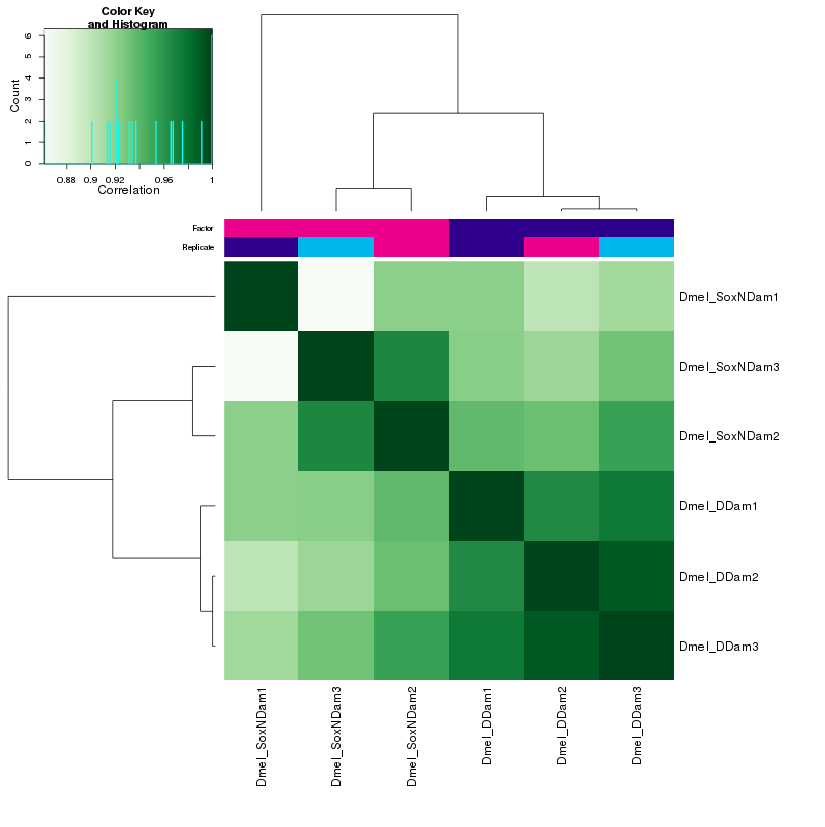
\includegraphics{fig4-8}
\caption{Clustering of \emph{D. melanogaster} Dichaete-Dam and SoxN-Dam samples by binding affinity scores in all bound intervals. Both the Dichaete-Dam replicates and the SoxN-Dam replicates cluster together, while the biggest outlier is SoxN-Dam replicate 1. The color key and histogram shows the distribution of correlation coefficients for affinity scores in each pair of samples. Darker green corresponds to a higher correlation between samples, while lighter green corresponds to a lower correlation.}
\label{Figure 4.8}
\end{figure}

Correlations between replicates for the same fusion protein range from 0.86 - 0.99, while correlations between replicates for different fusion proteins range from 0.90 - 0.95. Using DESeq2 normalization, DiffBind identifies 3001 intervals are that differentially bound between Dichaete-Dam and SoxN-Dam at FDR10 and 1048 at FDR1 (Figure 4.9). The FDR1 differentially bound intervals represent 5.0\% of all Dichaete-Dam bound intervals and 4.6\% of all SoxN-Dam bound intervals. Of the 1048 FDR1 intervals, 675 are preferentially bound by Dichaete-Dam and 373 are preferentially bound by SoxN-Dam.\\

\begin{figure}
\centering
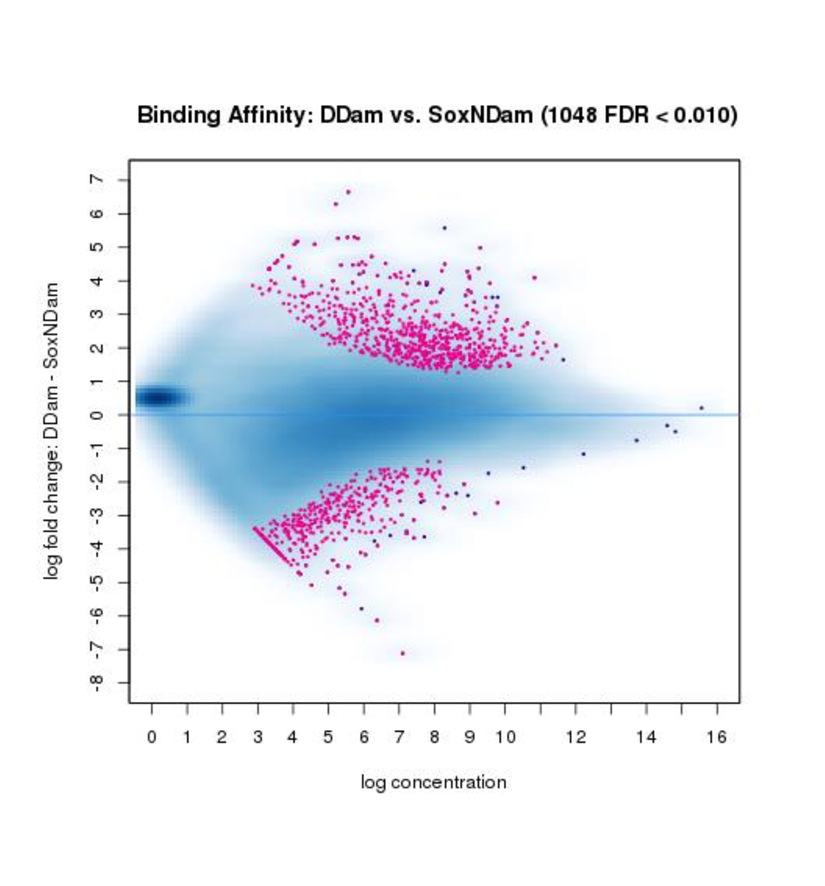
\includegraphics{fig4-9}
\caption{MA plot showing differentially bound intervals with FDR \textless 0.01 between \emph{D. melanogaster} Dichaete-Dam and SoxN-Dam. All intervals are plotted; differentially bound intervals are highlighted in pink.} 
\label{Figure 4.9}
\end{figure}

All of the intervals that are differentially bound by Dichaete-Dam were called as bound by Dichaete in the single-factor DESeq2 analysis. 459 of these were also called as bound by SoxN-Dam, while 216 were unique to Dichaete-Dam. All but one of the 373 intervals differentially bound by SoxN-Dam were called as bound by SoxN in the single-factor DESeq2 analysis, and of these, 114 were also bound by Dichaete-Dam, while 258 were unique to SoxN-Dam. The difference between the pattern of preferential binding by Dichaete-Dam and preferential binding by SoxN-Dam can be seen in a clustering of differential intervals by the log of normalized read counts within each interval (affinity score); many of the intervals preferentially bound by Dichaete-Dam are also strongly bound by SoxN-Dam, while a higher proportion of the intervals preferentially bound by SoxN-Dam are not bound or are weakly bound by Dichaete-Dam (Figure 4.10).\\

\begin{figure}
\centering
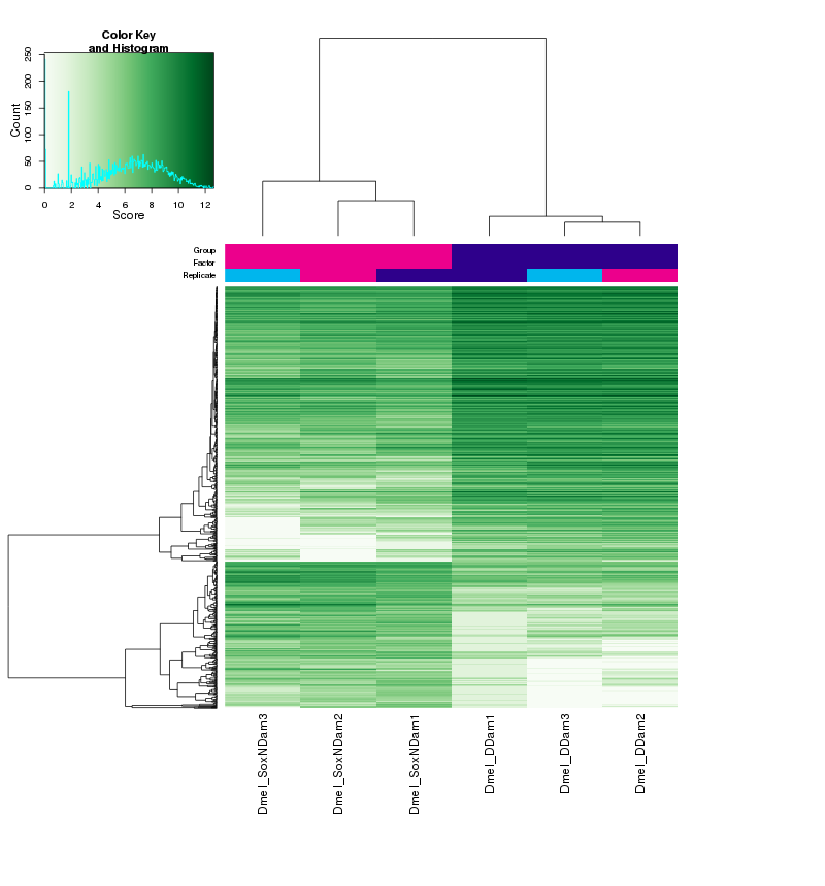
\includegraphics{fig4-10}
\caption{Clustering of \emph{D. melanogaster} Dichaete-Dam and SoxN-Dam differentially bound intervals by binding affinity scores. A block of intervals that are bound more highly by Dichaete is present in the upper right quadrant, while a block of intervals that are bound more highly by SoxN is present in the lower left quadrant. The color key and histogram shows the distribution of binding affinity scores (log of normalized read counts), in all bound intervals in each sample. Darker green corresponds to higher affinity scores or stronger binding, while lighter green corresponds to lower affinity scores or weaker binding.}
\label{Figure 4.10}
\end{figure}

In \emph{D. simulans}, a total of 19661 intervals are bound by Dichaete-Dam, SoxN-Dam, or both. In comparison to \emph{D. melanogaster}, the \emph{D. simulans} SoxN-Dam binding profiles within these intervals are much more similar to each other and more different from the Dichaete-Dam binding profiles. The correlations between replicates for the same fusion protein range from 0.91 - 0.98, and the correlations between replicates for different fusion proteins range from 0.47 - 0.62 (Figure 4.11). In agreement with the lower correlations between Dichaete-Dam and SoxN-Dam binding profiles, a DiffBind analysis with DESeq2 normalization identified many more differentially bound intervals between Dichaete and SoxN in \emph{D. simulans} than in \emph{D. melanogaster}. 8807 differential binding intervals were identified at FDR10, and 4881 were identified at FDR1 (Figure 4.12). The FDR1 differentially bound intervals represent 30.3\% of all Dichaete binding intervals and 32.2\% of all SoxN binding intervals. Of the 4881 FDR1 intervals, 2294 are preferentially bound by Dichaete-Dam, while 2587 are preferentially bound by SoxN-Dam. All but one of the intervals called as preferentially bound by Dichaete-Dam were identified as bound intervals in the single-factor DESeq2 analysis. Of these, 782 were also called as bound by SoxN-Dam, while roughly twice as many, 1511, were unique to Dichaete-Dam. All of the intervals called as preferentially bound by SoxN-Dam were identified as bound intervals in the single-factor DESeq2 analysis. 1502 of these were also called as bound by Dichaete-Dam, while 1085 were unique to SoxN-Dam. This is in contrast to the \emph{D. melanogaster} data, where the majority of the SoxN-Dam differentially bound peaks were unique to SoxN-Dam. This pattern can clearly be seen in a heatmap clustering differentially bound sites by affinity score (Figure 4.13).\\

\begin{figure}
\centering
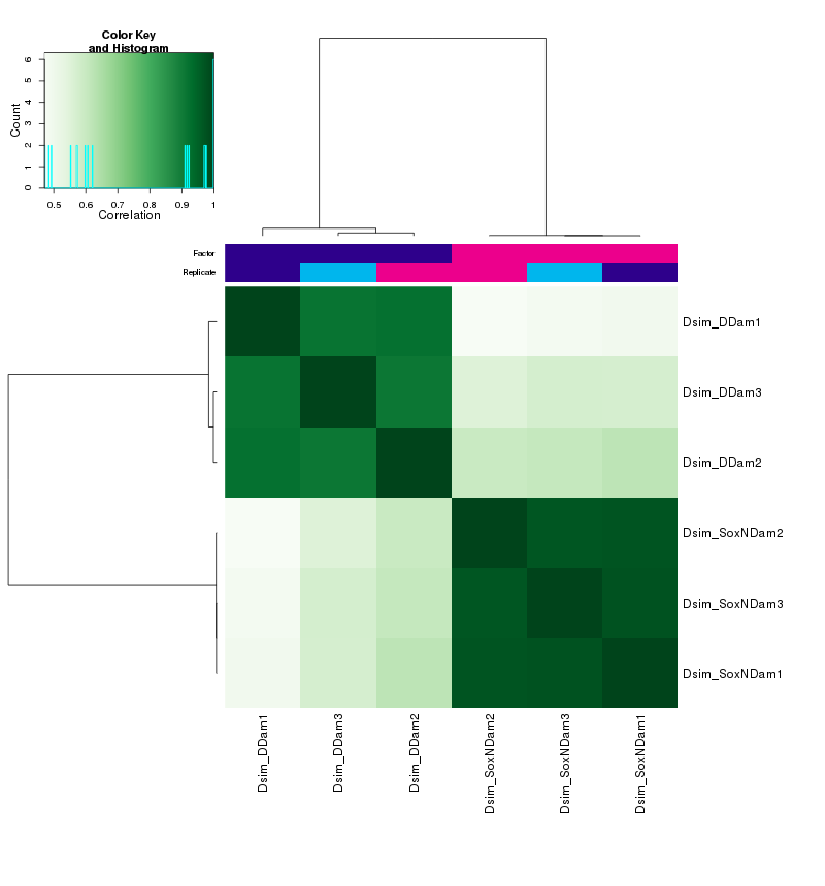
\includegraphics{fig4-11}
\caption{Clustering of \emph{D. simulans} Dichaete-Dam and SoxN-Dam samples by binding affinity scores in all bound intervals. Both the Dichaete-Dam replicates and the SoxN-Dam replicates cluster strongly together. There is a greater differentiation visible between the two transcription factors than in \emph{D. melanogaster}. The color key and histogram shows the distribution of correlation coefficients for affinity scores in each pair of samples. Darker green corresponds to a higher correlation between samples, while lighter green corresponds to a lower correlation.}
\label{Figure 4.11}
\end{figure}

\begin{figure}
\centering
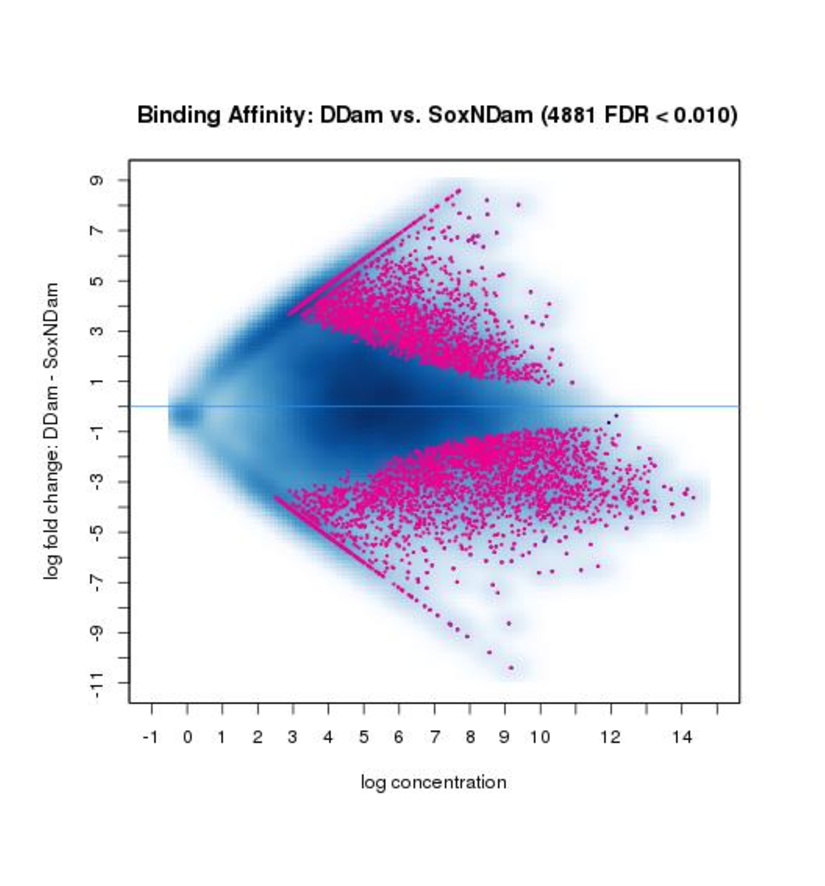
\includegraphics{fig4-12}
\caption{MA plot showing differentially bound intervals with FDR \textless 0.01 between \emph{D. simulans} Dichaete-Dam and SoxN-Dam. All intervals are plotted; differentially bound intervals are highlighted in pink.}
\label{Figure 4.12}
\end{figure}

\begin{figure}
\centering
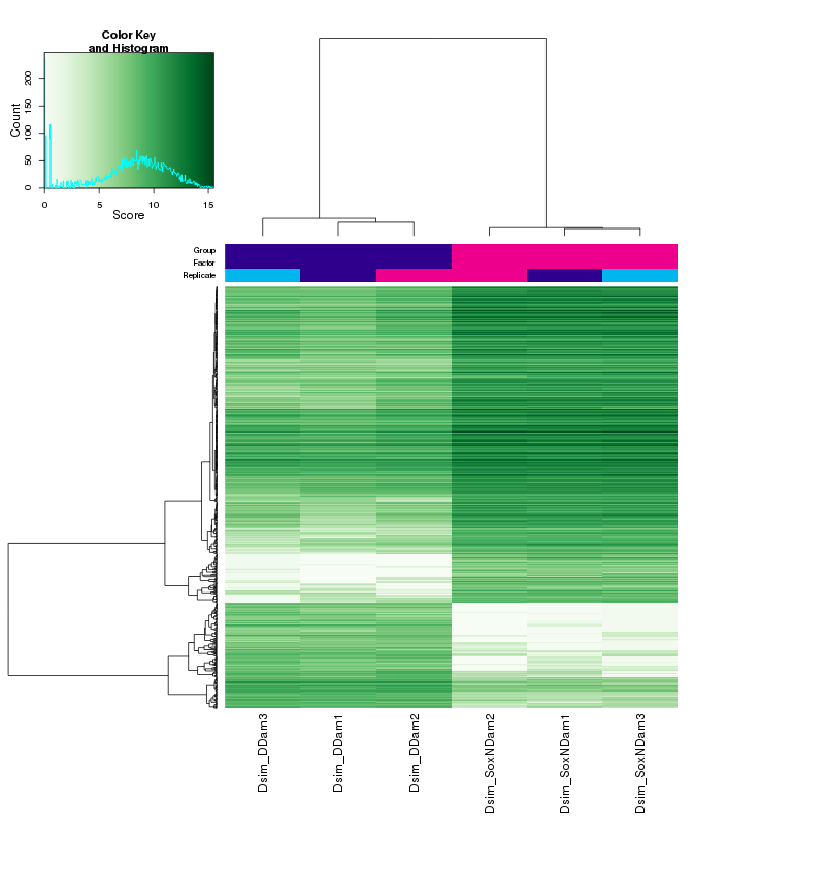
\includegraphics{fig4-13}
\caption{Clustering of \emph{D. simulans} Dichaete-Dam and SoxN-Dam differentially bound intervals by binding affinity scores. A block of intervals that are bound more highly by Dichaete is present in the lower left quadrant, while a block of intervals that are bound more highly by SoxN is present in the upper right quadrant. A greater number of intervals are more highly bound by SoxN than by Dichaete, which is the opposite of the case in \emph{D. melanogaster}. The color key and histogram shows the distribution of binding affinity scores (log of normalized read counts), in all bound intervals in each sample. Darker green corresponds to higher affinity scores or stronger binding, while lighter green corresponds to lower affinity scores or weaker binding.}
\label{Figure 4.13}
\end{figure}

There are some notable differences between the patterns of Dichaete and SoxN binding in the \emph{D. melanogaster} data as opposed to the \emph{D. simulans} data. The binding profiles of Dichaete and SoxN are more highly correlated in \emph{D. melanogaster} than in \emph{D. simulans}, which is a surprising finding. Accordingly, a much larger number of sites that are differentially bound between the two proteins was identified in \emph{D. simulans} than in \emph{D. melanogaster}. Figure 4.14 shows an example of a region where there are more differentially bound intervals between SoxN and Dichaete in \emph{D. simulans} compared to \emph{D. melanogaster}. It should be recognized that, while using DiffBind to examine differences in each species permits normalization of the Dichaete-Dam and SoxN-Dam data within each species to each other, it does not allow for normalization of the data between species, meaning that the thresholded intervals called as differentially bound in each species are not directly comparable. Nonetheless, examining the binding profiles shows that there are differences between the ways in which the two TFs bind relative to one another in the two species, which can be compared on an overall level; this question will be revisited in more detail in Chapter 5.\\

\begin{figure}
\centering
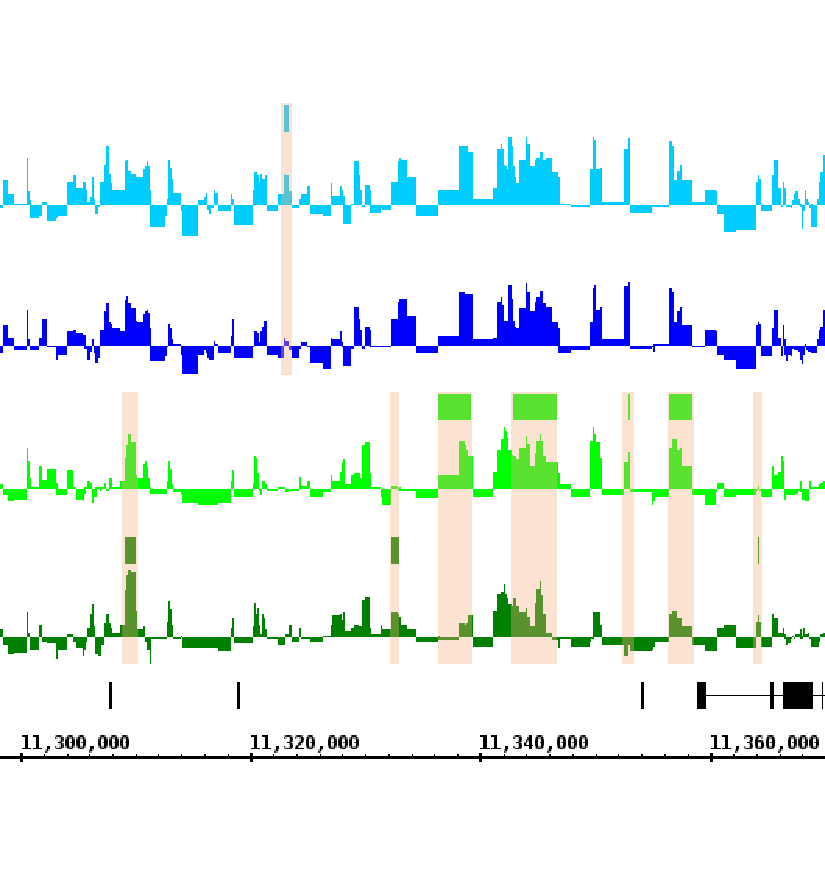
\includegraphics{fig4-14}
\caption{Quantitative differences in binding by Dichaete-Dam and SoxN-Dam in \emph{D. simulans} versus in \emph{D. melanogaster}. From the bottom, the \emph{D. simulans} Dichaete-Dam binding profile is in green, the \emph{D. simulans} SoxN-Dam binding profile is in light green, the \emph{D. melanogaster} Dichaete-Dam binding profile is in blue and the \emph{D. melanogaster} SoxN-Dam binding profile is in light blue. Intervals that are differentially bound by one TF in each species are represented by color-coded blocks above each respective binding profile. Three intervals that are preferentially bound by SoxN in \emph{D. simulans} but not in \emph{D. melanogaster}, as well as four intervals that are preferentially bound by Dichaete in \emph{D. simulans} but not in \emph{D. melanogaster}, are shown. In the same region, only one interval is preferentially bound by SoxN in \emph{D. melanogaster} and none are preferentially bound by Dichaete. All intervals that are preferentially bound by one TF in comparison to the other are highlighted in tan.}
\label{Figure 4.14}
\end{figure}

For each species, I assigned the intervals that are preferentially bound by either Dichaete or SoxN, as well as those that are uniquely bound by either Dichaete or SoxN, to the closest gene within 10 kb upstream or downstream. The preferentially bound and uniquely bound intervals are not mutually exclusive; rather, the uniquely bound intervals are a subset of the preferentially bound intervals. In \emph{D. melanogaster}, this resulted in 826 genes that are preferential targets of Dichaete and 251 that are unique targets of Dichaete, as well as 498 genes that are preferential targets of SoxN and 371 that are unique targets of SoxN. In \emph{D. simulans}, 2180 genes are preferential and 1507 are unique targets of Dichaete, while 2295 genes are preferential and 995 are unique targets of SoxN. I then analyzed the resulting lists of target genes using FlyMine \citep{lyne_flymine:_2007}. The GO:BP term enrichments are quite similar for both the preferential and unique targets of each transcription factor in each species. In \emph{D. melanogaster}, SoxN targets are broadly enriched for terms relating to development and biological regulation. Dichaete targets are also enriched for developmental terms, but, additionally, they show enrichment for signalling (p \textless 0.02), cell communication (p \textless 0.02) and response to stimulus (p \textless 1e-20). Interestingly, the Dichaete unique targets also show enrichment for synapse assembly (p = 0.013) and synaptic transmission (p = 0.023). In \emph{D. simulans}, both Dichaete and SoxN targets are highly enriched for developmental terms (p \textless 1E-11), but Dichaete targets have higher enrichments for imaginal disc morphogenesis (p \textless 1E-8), while SoxN targets have higher enrichments for terms related to the regulation of transcription (p \textless 1E-31). In both species, the Dichaete targets tend to be upregulated in the brain, head, hindgut, larval hindgut and larval CNS according to the FlyAtlas expression data, while the SoxN targets are only highly upregulated in the larval CNS and, in \emph{D. melanogaster}, the ovary.

\section{Discussion of results}
In this chapter I have presented the major datasets that I generated during my Ph.D., using DamID-seq to measure in vivo genome-wide binding of the two group B Sox proteins Dichaete and SoxN in four species of \emph{Drosophila}. This approach was successful in \emph{D. melanogaster} and \emph{D. simulans}, the two most closely-related species in my study. In \emph{D. yakuba}, I successfully generated a high-quality in vivo binding profile for Dichaete; however, the DamID experiment for SoxN in this species failed, likely due to a mutation rendering the SoxN portion of the fusion protein nonfunctional. In \emph{D. pseudoobscura}, I was unable to generate a transgenic line for SoxN-Dam, despite multiple injection attempts. The Dichaete-Dam experiment in this species was successful in that it uncovered binding intervals that show multiple indications of being biologically functional in vivo; however, the higher variance observed between replicates in comparison to other species resulted in significantly less binding intervals being called. Given the highly similar expression and sequence data for Dichaete between \emph{D. pseudoobscura} and the other species studied, it is unlikely that this reflects any underlying biological difference in Dichaete function. The amino acid sequences of the HMG-box DNA-binding domains of Dichaete are identical in \emph{D. melanogaster} and \emph{D. pseudoobscura}; however, there are some potentially significant differences in the N- and C-terminal regions \citep{mckimmie_conserved_2005}. It is possible that these differences are responsible for the increased variability in binding observed when the \emph{D. melanogaster} protein is expressed in \emph{D. pseudoobscura}, as the fusion protein may have a reduced ability to have its binding stabilized through interactions with cofactors compared to the endogenous Dichaete. Nonetheless, these datasets represent the first assay of group B Sox binding in \emph{Drosophila} species other than \emph{D. melanogaster} and, to my knowledge, the first time that DamID-seq has been used in a comparative binding experiment.\\ 

I used multiple types of analyses to assess the functionality of the identified binding intervals, including discovery of de novo and known TF binding motifs, annotation to genes and genomic features, overlap with previously defined high-confidence \emph{D. melanogaster} core intervals for each TF, overlap with known \emph{D. melanogaster} enhancers, and gene ontology enrichment analysis of potential target genes. For each dataset in each species, these analyses show good agreement with previous group B Sox binding data and indicate that the binding intervals are likely to represent true instances of gene regulation by Dichaete and SoxN. In \emph{D. pseudoobscura}, the Dichaete-Dam binding intervals show much lower overlap with known enhancers, and their putative target genes show lower overlap with direct target genes or targets of core binding intervals, than in other species. However, this is likely to be at least partially due to the much lower number of binding intervals identified overall; both the motif and Gene Ontology enrichments show good indications of known Dichaete function.\\

On a broad scale, the binding patterns that I identified for Dichaete-Dam and SoxN-Dam indicate that the functions of these proteins are largely conserved among the \emph{Drosophila} species studied. There are no notable differences between species in the enriched GO:BP terms identified in sets of genes associated with Dichaete-Dam or SoxN-Dam binding intervals, suggesting that the two TFs have maintained their roles in early CNS specification, neural development and morphogenesis, and regulation of other developmentally important transcription factors. Several verified Dichaete target genes are identified in \emph{D. simulans, D. yakuba} and \emph{D. pseudoobscura}, including \emph{nubbin (nub), grainy head (grh), miranda (mira)} and \emph{POU domain protein 2 (pdm2)}, which are involved in maintenance of neuroblast self-renewal as well as differentiation; \emph{decapentaplegic (dpp), wingless (wg), brother of odd with entrails limited (bowl), drumstick (drm), bagpipe (bap), Delta (Dl), outstretched (os), faint sausage (fas)} and \emph{ribbon (rib)}, which are targets of Dichaete in the hindgut; and \emph{slit (sli)}, a Dichaete target in the midline \citep{aleksic_role_2013}. Similarly, direct targets of SoxN that are conserved in \emph{D. simulans} include the proneural gene \emph{asense (ase)} and the proneural repressor \emph{hairy (h)}; \emph{Drop (Dr)}, a gene involved in DV patterning in the CNS; \emph{Kruppel (Kr), nub, pdm2, castor (cas), inscuteable (insc), numb, sanpodo (spdo), snail (sna), worniu (wor)}, and \emph{escargot (esg)}, which are involved in specifying neuroblast identity and controlling neuroblast self-renewal and asymmetric divisions \citep{buescher_binary_1998,cai_family_2001,isshiki_drosophila_2001,kraut_role_1996,maurange_brainy_2005,oconnor-giles_numb_????,skeath_sanpodo_1998,van_doren_negative_1994}; and \emph{cut (ct), dawdle (daw), knot (kn), longitudinals lacking (lola), midline (mid), nervous fingers 1 (nerfin-1)} and \emph{Sema-1a}, all SoxN targets involved in morphogenesis of axons and dendrites \citep{ferrero_soxneuro_2014,giniger_lola_1994,jinushi-nakao_knot/collier_????,kuzin_nerfin-1_2005,liu_midline_2009,parker_divergent_2006,yu_transmembrane_????}.\\

As with many other developmentally important regulators, Dichaete and SoxN bind extensively across the genome in all species studied. It has previously been suggested that Dichaete can bind at highly occupied target (HOT) regions in the \emph{D. melanogaster} genome, where it may facilitate the formation of complexes of other regulatory factors by causing DNA bending \citep{aleksic_role_2013}. I found a highly enriched motif for Trl, a marker of HOT regions, in both Dichaete-Dam and SoxN-Dam binding intervals, indicating that both proteins may be able to play this role. Several motifs for potential cofactors of Dichaete and SoxN were also enriched in binding intervals in multiple species. A motif for the known Dichaete cofactor Vvl is enriched in both the \emph{D. melanogaster} and \emph{D. yakuba} Dichaete-Dam binding intervals, as well as the \emph{D. simulans} SoxN-Dam binding intervals. A motif for Vnd, a transcription factor that plays an important role in the specification of the CNS \citep{ferrero_soxneuro_2014,zhao_sox-domain_2002}, is enriched in Dichaete-Dam binding intervals in both \emph{D. yakuba} and \emph{D. pseudoobscura}. Dichaete binding has been shown to overlap significantly with Twi and Kni binding in \emph{D. melanogaster} \citep{aleksic_role_2013}; a Twi motif was also found to be enriched in the \emph{D. pseudoobscura} Dichaete-Dam binding intervals, while a Kni motif was found to be enriched in the \emph{D. simulans} as well as the \emph{D. melanogaster} Dichaete-Dam binding intervals. Tll is a target of Dichaete in the hindgut and may work with it to regulate hindgut development \citep{aleksic_role_2013}; a tll motif is enriched in Dichaete-Dam binding intervals in \emph{D. simulans} and \emph{D. yakuba}, as well as in SoxN-Dam binding intervals in \emph{D. melanogaster} and \emph{D. simulans}. Taken together, these results suggest that the transcriptional networks in which Dichaete and SoxN are embedded are also highly conserved between \emph{Drosophila} species.\\

Although DamID-seq provides less spatial resolution and accuracy in measuring TF binding than ChIP-seq, because the distribution of bound fragments depends on the distribution of GATC sites in the genome, rather than on randomly sheared chromatin, certain features of Dichaete and SoxN binding patterns can be observed from the DamID-seq datasets. In all species studied, both proteins show a tendency to bind in introns; this is evidenced both by the high percentages of binding intervals that are annotated directly to introns and the downstream skew of binding intervals relative to TSSs. This pattern appears to hold across all species, although Dichaete-Dam binding intervals in \emph{D. pseudoobscura} show a higher tendency to be annotated to intergenic regions than in other species. Both Dichaete-Dam and SoxN-Dam intervals also show high overlaps with known functional enhancers. These two enrichments are not mutually exclusive, as many developmentally important enhancers in \emph{Drosophila} are known to be located within introns, including the enhancer to which Dichaete has been shown to bind in the midline gene \emph{sli} \citep{aleksic_role_2013,ma_functional_2000}. The STARR-seq enhancers which are bound by Dichaete and SoxN in \emph{D. melanogaster} and \emph{D. yakuba} are found near genes that are enriched for similar functions as the general sets of target genes for Dichaete and SoxN binding, providing evidence that binding at these loci is not incidental but is linked to regulatory function.\\

Using the data generated in \emph{D. melanogaster} and \emph{D. simulans}, I have also investigated the similarities and differences between Dichaete and SoxN binding patterns in two species. Prior to this work, it was known that Dichaete and SoxN showed highly similar patterns of binding \emph{in vivo} in \emph{D. melanogaster}, yet that their binding patterns were not identical \citep{ferrero_soxneuro_2014}. My datasets confirm this view. Generally speaking, the substantial overlap between Dichaete and SoxN binding that was observed in \emph{D. melanogaster} is a conserved feature of group B Sox binding in \emph{D. simulans}. However, somewhat surprisingly, the preliminary analysis of Dichaete and SoxN binding suggests they may be more differentiated in \emph{D. simulans}, both at the level of sequencing read correlations and binding interval locations. Since the fusion proteins expressed in both species were identical and derived from the gene sequences of \emph{D. melanogaster}, any difference between species must be due to differences in the nuclear environment in \emph{D. simulans}; that is, either sequence changes in \emph{cis}-regulatory elements where Dichaete and SoxN bind or changes in \emph{trans} affecting the overall transcriptional regulatory network. While it is possible that Dichaete and SoxN function in a more independent manner in \emph{D. simulans} than in \emph{D. melanogaster}, one intriguing hypothesis is that the targets that are common to the two proteins in both species may be the sites of more functionally important binding events. Dichaete and SoxN recognize very similar sequence motifs, contributing to the similarity of their binding profiles; however, it is likely that not all of the observed binding events are functional. Perhaps expressing proteins from \emph{D. melanogaster} in \emph{D. simulans} allows for a de-coupling of functional binding and binding driven by incidental Sox motifs; this hypothesis should be tested in the future by performing transgenic assays of enhancer function. In the following chapter, I will examine the relationship between common and unique binding by Dichaete and SoxN in both species in greater depth.\\

Although these DamID binding datasets provide a rich resource for the comparative study of group B Sox binding, they also have some limitations. The material used for DamID, whole embryos from overnight collections, represented both a mix of various tissue types and a broad range of developmental stages. The binding intervals identified therefore reflect an average picture of group B Sox binding during development, rather than the exact binding profiles in any one cell type at a given time. As discussed previously the limit of spatial resolution possible with DamID is dependent on the location of GATC sites, making the exact identification of binding sites more difficult than with ChIP. Nonetheless, DamID can give a reasonably accurate view of binding patterns; the average binding interval lengths for these datasets range from 589 bp to 1474 bp, which are shorter than many relevant genomic features, such as genes or even introns. As with ChIP, DamID identifies all regions where the fusion protein binds \emph{in vivo}. However, these binding events may not all be functional in the sense of contributing to transcriptional activation or repression. It is possible to identify direct targets of a TF by combining \emph{in vivo} binding data with gene expression data in a mutant background, which has been done for Dichaete and SoxN in \emph{D. melanogaster}. However, these “functional” binding events typically only make up a fraction of the genes that are bound by a TF, raising the question of what the effect of binding at other loci is. Some of this binding may simply be due to the thermodynamic affinity of TFs for DNA \citep{biggin_animal_2011,fisher_dna_2012,kaplan_quantitative_2011}, although, for TFs like Dichaete and SoxN which can induce DNA bending, it might help create enhancer loops to bring other regulatory factors together \citep{ghavi-helm_enhancer_2014}. In this view, loss of Sox binding may result in variable effects on gene expression or increase expression noise due to perturbation of the regulatory network, both difficult to detect with standard genomic expression analysis. Such a role, and observed variable effects on gene expression, have been reported for Dichaete \citep{russell_dichaete_1996}. One way to more specifically address this question is to examine which binding events have been conserved during evolution, as functional binding is more likely to be constrained by natural selection \citep{biggin_animal_2011}.\\

In general, the genomic features associated with Dichaete and SoxN binding, including sequence motifs and putative gene targets, appear to be quite similar between species of \emph{Drosophila}. This finding supports the expectation that Dichaete and SoxN have broadly similar roles during development across the drosophilids and, indeed, as far distant as vertebrates \citep{uwanogho_embryonic_1995-1,wood_comparative_1999}. However, a significant number of binding intervals differ between \emph{D. melanogaster} and the other species examined, raising the question of the evolutionary significance of these differences in binding patterns. Thus far, I have only performed a crude comparison of the binding patterns between different species. In the following chapter, I will dissect the differences and similarities in binding on a quantitative basis, including the relationships between Dichaete and SoxN binding, and examine the possible mechanisms of binding site turnover and evolution within the phylogenetic distances that I have studied.


